\usepackage[utf8]{inputenc}
\usepackage{pdfpages} % to prepend the title page
\usepackage{amsfonts}
\usepackage{amsmath}
\usepackage{subcaption}  % not sure if this is necessary
\usepackage[skip=10pt plus1pt, indent=0pt]{parskip} % skip space after paragraph and remove indent
\usepackage{csvsimple}
\usepackage{booktabs}
\usepackage{floatrow}
\usepackage{tocloft}
\usepackage[font={sf, small,it}]{caption} % change caption appearance
\usepackage{titlesec}
\usepackage[scaled]{helvet} % Scale Helvetica to match the size of the default font
\usepackage[T1]{fontenc}    % Ensure proper font encoding
\usepackage{lmodern}
\usepackage[backend=biber, style=apa, url=false, sorting=ynt]{biblatex} % citations
\usepackage{graphicx} % for images
\graphicspath{ {./images/} }

\renewcommand{\familydefault}{\sfdefault} % Set the default font to sans-serif (Helvetica)

\emergencystretch=2em % if a line is too long, allow 2em over

% code snippets style
\usepackage{listings}
\usepackage{xcolor}
\definecolor{bg}{HTML}{EEE5E9}
\definecolor{orange}{HTML}{CF5C36}
\definecolor{gray}{HTML}{7C7C7C}
\definecolor{codegray}{rgb}{0.5,0.5,0.5}
\definecolor{codepurple}{rgb}{0.58,0,0.82}
\lstdefinestyle{python}{
  basewidth={.5em,0.4em},
  backgroundcolor=\color{bg},   
  commentstyle=\color{gray},
  keywordstyle=\color{orange},
  numberstyle=\tiny\color{codegray},
  stringstyle=\color{codepurple},
  basicstyle=\ttfamily\footnotesize,
  breakatwhitespace=false,         
  breaklines=true,                 
  captionpos=b,                    
  keepspaces=true,                 
  numbers=left,                    
  numbersep=5pt,                  
  showspaces=false,                
  showstringspaces=false,
  showtabs=false,                  
  tabsize=4,
  %frame=shadowbox,
  xleftmargin=2em,
  frame=single,
  framexleftmargin=1.5em
}
\lstset{style=python}

% define headline styles
\titleformat{\chapter}[display]
  {\normalfont\sffamily\huge\bfseries}
  {\chaptertitlename\ \thechapter}{0pt}{\Huge}
\titleformat{\section}
  {\normalfont\sffamily\Large\bfseries}
  {\thesection}{1em}{}
\titleformat{\subsection}
  {\normalfont\sffamily\Large}
  {\thesubsection}{1em}{}
\titleformat{\subsubsection}
  {\normalfont\sffamily\large}
  {\thesubsubsection}{1em}{}

\addbibresource{bibliography.bib}


\begin{document}
\sffamily
\pagenumbering{roman}

% start of the thesis
\pagenumbering{arabic}
\chapter*{Abstract}
\addcontentsline{toc}{chapter}{Abstract}

The Lottery Ticket Hypothesis by \textcite{LTH} has sparked a novel field of research that focuses on finding well-trainable sparse neural networks.
\textit{Iterative Magnitude Pruning} is a central method in this field.
It successfully uncovers sparse subnetworks that achieve performance comparable to the original dense network when trained in isolation. 
These networks are called \textit{Winning Tickets}.
Why and how iterative magnitude pruning works and what characteristics of the winning tickets make them successful remain elusive.
To learn more about winning tickets, their network structure is studied in this thesis.
Since they are sparse subnetworks, their structure may contain valuable insights into their functionality.
Training data with a known structure is used to examine whether winning tickets trained on that data resemble its structure in any way.
The experiments in this thesis are conducted on datasets that contain two independent tasks \rule[0.5ex]{.5em}{0.5pt} a simple toy dataset and a combination of the MNIST and Fashion-MNIST datasets.
With both datasets, the resulting winning tickets resemble the structure of the datasets, namely the independence.
The winning tickets contain separate, independent subnetworks where each subnetwork solves one independent task.

\chapter*{Kurzfassung}
\addcontentsline{toc}{chapter}{Kurzfassung}

Die von \textcite{LTH} aufgestellte Lottery Ticket Hypothese hat einen neuen Teilbereich der Forschung begründet, der sich mit \textit{Sparse Neural Networks} beschäftigt, welche erfolgreich trainiert werden könne.
\textit{Iterative Magnitude Pruning} ist eine Schlüsselmethode für dieses Feld, da sie die schlanken und performanten Subnetzwerke, die sogenannten \textit{Winning Tickets} erfolgreich ausfindig machen kann.
Wieso diese Methode erfolgreich ist und was die Subnetzwerke, die \textit{Winning Tickets} so erfolgreich macht, ist großteils unerklärt.
Eine Möglichkeit um \textit{Winning Tickets} und deren Erzeugung besser zu verstehen, ist die Analyse des Netzwerkgraphens.
Dadurch, dass diese Subnetze \textit{sparse} sind, könnte ihre Struktur wertvolle Einblicke in die Funktion des Netzwerkes bieten.
Im Rahmen dieser Masterarbeit wird die Struktur der \textit{Winning Tickets} und ihre Verbindung zur Funktion des Netzes untersucht.
Dazu wurden Experimente auf Datensätzen mit unabhängigen Aufgaben erstellt \rule[0.5ex]{.5em}{0.5pt} ein einfacher synthetischer Datensatz und eine Kombination aus dem MNIST und dem Fashion-MNIST Datensatzes.
Mittels \textit{Iterative Magnitude Pruning} können für beide Datensätze unabhängige Subnetwzerke im \textit{Winning Ticket} gefunden werden, wobei jedes Subnetzwerk eine Aufgabe des Datensatzes löst.
\newpage
\tableofcontents
\chapter{Introduction}

Neural Networks have achieved remarkable success in various tasks, however, their increasingly large size leads to high computational and memory requirements.
The Lottery Ticket Hypothesis by \textcite{LTH} has shown that there exist small, well-initialized subnetworks that can be trained in isolation to reach the same accuracy as the larger dense networks.
These small subnetworks, the so-called \textit{Winning Tickets}, are created by iterative training and pruning a fully connected dense network.
This process is called \textit{Iterative Magnitude Pruning}.
The work by \textcite{LTH} defines a promising avenue towards the ability to train smaller sparse networks from the beginning.
However, a deep understanding of why the winning tickets can learn so well and why iterative magnitude pruning can uncover them is missing.

Although there is plenty of research in the field, the structure of the winning tickets is rarely discussed.
Since the winning ticket networks are sparse, their structure might give valuable insights into their functionality.
In this thesis, the structure of winning tickets is studied and how it relates to the function of the network.

\section{Motivation}
Understanding more about the structure of winning tickets can lead to numerous advances.
Studying it can generate insights about the algorithms like iterative magnitude pruning, that are used to generate the winning tickets.
Potential drawbacks of the algorithm can be discovered by analyzing weaknesses in the network structure.

Further, the structure could give insights into the function the network has learned.
Due to the high sparsity of winning tickets, the network structure might reflect the higher-level semantic structure of the learned function.
This in turn can be instrumental for network interpretation.
Winning tickets could be used to find substructures in the functions they learn, which in turn could improve the interpretability.

% Objective
The objective of this thesis is to find out more about the structure of winning tickets and whether they contain meaningful features.

\section{Research Questions and Scope}
The general research question that follows from the objective is: 
\begin{quote}
\textit{Do winning tickets contain meaningful structures?}
\end{quote}

This question serves as the main direction of the research.
Due to the generality of the question, it is narrowed down for this thesis to be approachable.
Only standard fully connected feed-forward neural networks are used to derive winning tickets.
To uncover the winning tickets, iterative magnitude pruning is employed.
This results in a narrower research question:

\begin{quote}
\textit{Do winning tickets of fully connected feed-forward networks derived with iterative magnitude pruning contain meaningful structures?}
\end{quote}

This thesis contains empirical research that aims to answer this very question.


\section{Structure of the Thesis}
In chapter~\ref{literature_review}, a literature review is conducted, where topics relevant to this thesis are described.

Chapter~\ref{chapter:method} explains the methodology.
The dataset, neural network architecture, and training process are outlined, as well as other algorithms used in the experiments.
Chapter~\ref{chapter:experiments}  walks through the experiments that were conducted during this thesis.
Further, the results are discussed and interpreted.
The thesis is concluded with a discussion and possible future research in this direction in chapter~\ref{chapter:conclusion}.
\chapter{Literature Review}\label{literature_review}
In this chapter, the prerequisites and related research are reviewed and discussed.
Neural network pruning and the lottery ticket hypothesis, as well as relevant follow-up work, are covered in detail.
Alternative methods to find winning tickets are also outlined.
Further, aspects of the winning ticket network itself are covered, such as the numerical characteristics of the parameters and the structure of the network graph.

\section{Neural Network Pruning}
The field of deep learning is largely responsible for the advances of modern machine learning applications.
With increasing amounts of available data and computational resources, the size of neural networks has increased drastically, as well as their performance.
However, this increase in size poses challenges in constrained environments.
Larger and deeper networks tend to require more memory and computational resources, which can be problematic for inference on constrained devices.
Also, larger models typically require more time and more energy for training as well as for inference.

Neural Network Pruning \autocite{LeCun, OptimalBrainSurgeon, HanEtAl15, PruningFiltersForEfficientConvets} has been proposed as a tool to reduce network size for inference while maintaining accuracy.
Pruning algorithms can reduce parameter count by up to 90 percent without harming accuracy.
\autocite{LeCun, OptimalBrainSurgeon, HanEtAl15, PruningFiltersForEfficientConvets}
Pruning can be done in a single step, where the network is trained once and then pruned.
It can also be done iteratively. 
The network is repeatedly trained and pruned over several iterations. 
It has been shown that iterative pruning can further reduce network size significantly whilst maintaining performance \autocite{HanEtAl15}.
The resulting sparse subnetwork can represent an equally accurate function with significantly fewer parameters. 
The question arises: If it can represent the function, why not train the sparse network directly?
\textcite{HanEtAl15} and \textcite{PruningFiltersForEfficientConvets} attempted to train the pruned networks from scratch after they have been randomly reinitialized.
With this approach, the subnetworks did not reach comparable accuracy to the unpruned networks.
These findings seemingly demonstrate the difficulty of training sparse neural networks.
An investigation into this apparent shortcoming of sparse networks was conducted by \textcite{LTH}.
The authors discover the phenomenon that the sparse neural networks they created can indeed train to comparable accuracy.
The condition for this to work is that they are not randomly reinitialized. 
Instead, the respective values at initialization of the unpruned network are assigned to the remaining weights of the pruned network. 
Based on this finding, the authors formulate the \textit{Lottery Ticket Hypothesis}.

\section{The Lottery Ticket Hypothesis}\label{sec:lth}
The basis of the field of lottery tickets is the work of~\cite{LTH}. 
They show that dense neural networks consistently contain subnetworks that can be trained in isolation to comparable accuracy.
They find these well-performing subnetworks, which they call \textit{winning tickets}, in a variety of scenarios.
They are found with fully connected neural networks on the MNIST dataset~\autocite{mnist} and with convolutional neural networks~\autocite{cnn} on the CIFAR-10 dataset~\autocite{cifar}.
Further, they are found with different optimizers and different regularization techniques.
Based on these findings, the authors propose:

\begin{quote}
\textbf{The Lottery Ticket Hypothesis}: \textit{A randomly-initialized, dense neural network contains a subnetwork that is initialized such that—when trained in isolation—it can match the test accuracy of the original network after training for at most the same number of iterations.}~\cite{LTH}
\end{quote}

The authors primarily use a method called \textit{Iterative Magnitude Pruning} ({IMP}).
The state of the network at initialization is stored.
Then, the network is trained to convergence. 
After training, a fixed percentage of weights with the lowest magnitudes is pruned (set to zero).
Following the pruning step, the unpruned parameters of the network are reset to the values they had at initialization.
This process of training, pruning and resetting is repeated iteratively until the final desired sparsity is reached.
The result is a sparse subnetwork and, if it can be trained to comparable performance,  a \textit{winning ticket}.

The experiments of \autocite{LTH} show that iterative magnitude pruning as described above suffices for finding winning tickets in small architectures.
Concretely, for LeNet-{300}-{100}~\autocite{cnn} (which will be further referred to as LeNet) and convolutional neural networks that are smaller variants of VGG \autocite{SimonyanZisserman}.

Experiments were also conducted on larger, more commonly used networks for CIFAR-10. For {IMP} to obtain winning tickets in VGG-19 \autocite{Liu19} and ResNet-18 \autocite{ResidualConnect}, the following adaptations were required. 
\begin{enumerate}
  \item Pruning is no longer done layer-wise but globally, as it results in smaller winning tickets. 
  \item Learning rate warm-up is employed. The learning rate increases linearly from 0 to the specified final learning rate in the first $k$ iterations. For VGG-19 and ResNet-18, $k$ is 10000 and 20000 respectively.
\end{enumerate}
In follow-up work by \textcite{LinearModeConnectivity}, the authors address the problems that arise at scale.
Experiments done by \textcite{Liu19, Gale19} show that in more challenging settings, subnetworks obtained with {IMP} do not perform better than randomly sampled subnetworks.
To understand this phenomenon, \textcite{LinearModeConnectivity} propose a tool for understanding the failings of {IMP} in uncovering winning tickets.
For that, the authors introduce \textit{Instability Analysis}.

Instability refers to the network being susceptible to noise of Stochastic Gradient Descent (SGD).
SGD introduces noise by stochastically selecting the order of mini-batches for the network training.
To determine if a network is stable to this noise, first, the network has to be duplicated.
The two identical networks are then trained with different SGD noise, realized with different random seeds.
After training, there are two sets of weights, $\theta_A$ and $\theta_B$.
Between both sets of weights, a linear path is defined.
Along this path, the weights are linearly interpolated with $\theta_\alpha = \alpha \theta_A + (1 - \alpha \theta_B)$, where $\alpha \in (0,1)$. 
For each of the interpolated sets of weights $\theta_\alpha$, the performance, or error, is measured.
The highest increase in the error of the interpolated weight sets $\theta_\alpha$ relative to the mean of the error of the original weights $\theta_A$ and $\theta_B$ is called the \textit{error barrier height}. 
If the error barrier height is smaller than a specified threshold, the network is considered linear mode connected and, hence, \textit{stable}.
The authors use a threshold of 2 percent as the threshold in their experiments, intended to tolerate noise. 
The implementation of the linear interpolation between the two weight sets is realized with 30 evenly spaced values of $\alpha$.

\textcite{LinearModeConnectivity} conduct instability analysis on unpruned dense networks with different architectures and datasets at initialization as well as during training.
For this experiment, they examined LeNet trained on MNIST, ResNet-20 and VGG-16 trained on CIFAR-10 as well as ResNet-50 and Inception-v3 \autocite{inceptionv3} on ImageNet~\autocite{imagenet}. 
They find that only LeNet is stable at initialization, however all other networks become stable early in training.
Furthermore and more interestingly, the authors conduct instability analysis on subnetworks uncovered by {IMP}.
In Addition, for this purpose the {IMP}-algorithm is generalized to rewind the weights to any step $k$ in training.

As described in this paragraph, the network state at initialization is saved in order to reset the network after pruning, which represents $k=0$.
This notion is generalized to any step $k$, where the state of the network after $k$ update steps is stored for resetting.
Networks derived with {IMP} and $k > 0$ are technically not winning tickets, since the condition for them is that the parameters are from initialization, meaning $k=0$.
Networks with parameters from later steps $k > 0$ are called \textit{matching}~\autocite{LinearModeConnectivity}.

The instability analysis at initialization shows that the subnetworks are only stable if they match.
Subsequently, the authors apply instability analysis to multiple subnetworks created from the same dense network over multiple values for the reset step $k$.
These experiments show that the subnetworks that are not stable when $k=0$ become stable when they are rewound to a later step $k$.
The step $k$ when they get stable closely coincides with the step where the subnetworks become matching, which suggests a tight link between the two concepts.
The experiments were only done with dense networks and extremely sparse networks, namely between 1.5\% and 16.8\% for the smaller networks, 30\% for ResNet-50, and InceptionNet \autocite{LinearModeConnectivity}.

\subsection{Pruning Strategies}
The original lottery ticket experiments use a simple pruning strategy of masking a certain percentage of weights with the lowest magnitudes \autocite{LTH}, as in \autocite{HanEtAl15}. This simple heuristic has yielded impressive results, yet there are many other possible heuristics one could imagine for such a task.
\textcite{Supermasks} perform an ablation study concerning pruning strategies. Mask criteria are defined as functions that determine a score for each parameter. This score is used to rank the parameters and the bottom $p\%$ are set to zero.
A variety of criteria is considered, including: 
\begin{itemize}
\item \textbf{Magnitude at initialization:} Mask the smallest (or largest) weights by their magnitude at initialization
\item \textbf{Magnitude after training:} Mask the smallest (or largest) weights by their magnitude after training
\item \textbf{Magnitude at initialization and after training:} Mask the weights that had the smallest (or largest) magnitudes at initialization and after training
\item \textbf{Magnitude increase:} Mask the weights that have the highest decrease or smallest increase in magnitude after training
\item \textbf{Movement:} Mask the weights that, after training, are closest to the value at initialization
\item \textbf{Random:} Mask randomly as a baseline for comparison
\end{itemize}
The authors followed the experimental setup of \textcite{LTH} and evaluated fully connected networks as well as convolutional neural networks.
The simple magnitude pruning approach is among the best performing in the experiments.
However, also pruning by movement produced well-performing winning tickets.
The results suggest that pruning the lowest magnitude weights of a network is a competitive strategy.
Although it may not be the best strategy, as other alternatives produce competitive results, it is a relevant algorithm to use and study. 

\subsection{Theory of Iterative Magnitude Pruning}
\textcite{WhyLotteryTicketsWin} hypothesize that winning tickets effectively relearn the same solution as the one achieved by pruning alone, which they term \textit{pruned solution}.
The authors show that the winning ticket subnetworks are significantly more similar to the pruned solution than they are to a trained but randomly reinitialized sparse network.
The experiments are conducted on the original LeNet architecture trained on the MNIST dataset, as well as ResNet-50 Architecture trained on ImageNet. Further, they show that the trained winning tickets reside in the same basin of the loss landscape as the pruned solution, by linearly interpolating between the two networks, in the same way as in \autocite{LinearModeConnectivity}.

\textcite{maene_towards_2021} name the hypothesis of \autocite{WhyLotteryTicketsWin} the regurgitating tickets interpretation.
They designed an experiment in which they forced the network to learn a different solution by creating a repellent loss function.
This loss increases when the model is close to the same solution as in the previous iteration of {IMP}.
This forces the network to find a new solution every iteration.
With the repellent loss, no winning tickets could be found, which further indicates that the solution found with {IMP} indeed relearns the pruned solution.

\section{Alternative Ways to Find Winning Tickets}
\subsection{Supermasks}
\textcite{Supermasks} demonstrate that it is possible to find well-performing subnetworks at initialization by only pruning.
First, each weight in the network is assigned a score, which is 1 for every weight at the beginning. 
The scores are denoted $s$.
In each forward pass of the network, the so-called \textit{effective weights} are used.
The effective weights $\theta_{eff}$ are the weights at initialization $\theta$ multiplied element-wise with a stochastically sampled mask.
This mask is sampled according to $m = \textit{Bern}(\sigma(s))$, where $\textit{Bern}(p)$ is a Bernoulli sampler producing a $1$ with probability $p$ and $\sigma(\cdot)$ is the sigmoid function. 
Thus, the effective weights are $\theta_{eff} = \textit{Bern}(\sigma(s)) \odot \theta$.
The scores are the learned parameters and are updated via backpropagation.
Experiments were conducted with a fully connected feed-forward neural network on MNIST and a convolutional network on CIFAR-10, reaching 95.3\% and 65.4\% test accuracy, respectively.
The authors call these masks \textit{supermasks}.

\subsection{Edge Popup}
Based on the results of \autocite{Supermasks}, \textcite{EdgePopup} scaled up the experiments and modified the algorithm for producing the mask slightly.
They remove the stochastic sampling of the Bernoulli sampler, as they claim that the stochasticity limits the performance. 
Instead of sampling the mask values, a real-valued score is learned for each weight. 
The subnetwork is chosen by selecting the top-$k$\% highest scores in each layer.
The algorithm for finding this mask is named \textit{Edge-Popup} (EP).
Experiments are conducted on small fully connected and convolutional neural networks with CIFAR-10 and several ResNet architectures with ImageNet.
Results show that even for the much harder ImageNet dataset, there exist randomly initialized subnetworks with non-trivial performance. 
An expressive finding of the experiments shows that a larger architecture (Wide-ResNet-50, 69M parameters) can reach 73.3\% accuracy on ImageNet by only pruning the weights with {EP}.
The resulting subnetwork has 20.6M parameters. In comparison, they show that this pruning-only approach can compete with a fully trained ResNet-34 (21.8M parameters) which also reaches 73.3\% accuracy. 
Surprisingly, the authors note that the subnetworks obtained by EP do not respond to any further training.
Furthermore, they note that the subnetwork does not train with the same accuracy as the dense network.
Therefore, the subnetworks are not considered winning tickets.
The results suggest that there is another phenomenon at play that makes these networks perform well \autocite{EdgePopup}.
Despite that, the experiments show that there exist well-performing subnetworks at initialization, without any weight updates.

\subsection{Rare Gems}
Drawing Inspiration from the EP-algorithm, \textcite{RareGems} propose an algorithm called Gem-Miner (GM) that overcomes the issues of the apparent lack of trainability of the obtained subnetworks.
The {GM}-algorithm assigns a normalized score to each weight. 
To obtain the mask $m$, a simple rounding function is applied to each score. The authors used a simple deterministic rounding function, where values below $0.5$ are rounded down to $0$ and all other values to $1$.
In the forward pass, the effective weights $\theta_{eff} = \theta \odot m$ are used, where $\theta$ are the untrained weights at initialization. 
The scores are the learned parameters and are updated via backpropagation.
Furthermore, the scores are renormalized to the range $[0,1]$ after they are updated, if necessary.
Additionally, a regularization term is added to the loss, which enforces sparsity on the scores. 
The authors use the $L_2$ norm of the scores and note that the $L_1$ norm performs almost identically.
The final sparsity of the obtained subnetwork can be controlled by the regularization hyperparameter $\lambda$, which scales the regularization term.
If $\lambda = 0$, there is no control over the final sparsity. 
The authors have discovered, in line with~\cite{EdgePopup}, that the sparsity level remains close to $50$ percent, as apparently, this is where the accuracy is maximized.

Experiments with different ResNet architectures on CIFAR-10, TinyImageNet \autocite{Tinyimagenet}, and Caltech-101 \autocite{Caltech101} were conducted. 
The results show that the subnetworks obtained via the {GM}-algorithm, are indeed winning tickets since they can then be trained and reach comparable accuracy to their dense counterpart.
Furthermore, the subnetworks have reasonably high accuracy \textit{before} any weight training, which earns them the name \textit{Rare Gems}. 
This makes the set of rare gems a subset of winning tickets. 
They are winning tickets, that already perform well before weight training.
The obtained subnetworks do not always outperform winning tickets obtained with {IMP}. 
However, there is a considerable improvement over {IMP} in terms of resource intensity.
The authors claim, that their algorithm is up to $19\times$ faster than the iterative approach with {IMP}. 
This increase in efficiency is compelling for repeated experiments.

\subsection{Pruning at Initialization}
In addition, a variety of other methods \autocite{GraSP, SNIP, SynFlow} were introduced to prune networks at initialization. 
However, empirical investigations by \textcite{PruningAtInitMissingTheMark, SanityCheckingPruningMethods} show that none of these approaches perform better than carefully selecting layer-wise sparsities.
Based on this finding, \autocite{SanityCheckingPruningMethods} propose a method that selects layer-wise sparsities called Smart-Ratio (SR).

\section{Analyzing Winning Tickets}
\subsection{Weight Distribution}
\textcite{maene_towards_2021} note that the average magnitude of the unpruned weights increases with each pruning round of {IMP}.
The smallest magnitude weights in the network are pruned, and the remaining weights train to similar values, thereby increasing the average magnitude.
In the original lottery tickets paper by \textcite{LTH}, the authors analyze the distribution of weight magnitudes after training.
Before the first pruning iteration, the distribution of weight magnitudes follows a Gaussian distribution, due to the networks initialization.
After several pruning iterations, the distributions tend towards a bimodal distribution, where the values close to zero are carved out.
The authors attempted to reinitialize the sparse subnetworks randomly according to the distribution of the lottery ticket weight magnitudes, however, the performance was only slightly better than reinitialization with the original weight distribution.
This hints at the fact, that the structure of the network graph is not the only necessary component to make lottery tickets work.

\subsection{Network Structure}
Even though the structure alone is not responsible for the success of the winning ticket, it might still be worth studying.
The structure of a neural network can viewed as a directed acyclic graph.
Since it is sparsely connected, the remaining connections could provide insight into the functionality of the network.
\textcite{LTH} analyze the connectivity of each node in the winning ticket network graph.
They find that the input connectivity, namely the number of incoming edges to a node (neuron) is relatively even among nodes of the same layer.
The input connectivity of each node in LeNet trained on the MNIST dataset is approximately proportional to the sparsity of the layer.
Regarding the output connections, there are bigger differences in connectivity amongst nodes.
Especially in the input layer, a significant proportion of nodes has no remaining outgoing connections at high sparsities.
The authors hypothesize that the disconnected input nodes are not informative and likely correspond to the outer frame of the MNIST image, which does not contain information about the desired prediction task.

When applying unstructured pruning (pruning individual weights instead of neurons), some neurons may end up in a state where they do not have any incoming or outgoing connections. 
\textcite{HanEtAl15} acknowledge the possibility of such neurons, which will be referred to as \textit{dead neurons}. 
According to \autocite{HanEtAl15}, the dead neurons do not contribute to the final loss and therefore do not receive any gradients. 
During retraining, regularization will remove the dead neurons automatically. 
A missing scenario is the existence of a neuron with outgoing connections, a bias, and no incoming connections. This neuron might still contribute to the output and receive gradients. 
In this case, the neuron is considered dead, but removing it changes the output of the network.
\textcite{AllAlivePruning} include this scenario and describe that removing such a neuron maintains the function of the network by simply transferring the bias to the next layer. 
Therefore, all neurons with no incoming or outgoing connections can safely be considered dead, thus removable. 
Further, all weights connected to a dead neuron can be removed as well.
\textcite{AllAlivePruning} propose a novel pruning strategy that makes use of this knowledge, named \textit{All-Alive-Pruning}. 
The authors use iterative magnitude pruning, similar to \autocite{LTH}.
Dead neurons and the weights connected to them are removed after pruning, resulting in an \textit{all-alive} network.
Only at very high sparsities, the networks pruned with All-Alive-Pruning demonstrate improved performance. 
This improvement is attributed to the increased capacity of the subnetwork since more of its parameters are \textit{alive} and can contribute to the network output.

Only a few researchers looked at winning tickets derived with iterative magnitude pruning as sparsely connected graphs. 
The insights relate the function of the network to its structure.
Dead neurons \autocite{HanEtAl15, AllAlivePruning} are neurons that are part of the graph structure that can be removed without harming the function.
\textcite{LTH} discover that inputs that do not transmit information are pruned at higher rates, leaving them with fewer outgoing connections.
Overall the structure of winning tickets and how it relates to its function remains elusive.

\section{Brain-Inspired Modular Training}
A sparse network where the structure of the network relates to the underlying algorithm or problem structure can be beneficial for interpretability.
\textcite{BIMT} propose a training method called Brain-Inspired Modular Training (BIMT) that aims to produce sparse networks that can more easily be visually interpreted.
The authors aim to encourage modularity in the network by embedding the neurons in an Euclidean space.
By punishing connections that are long in Euclidean space, visible clusters of neurons form. 
Since neurons that are next to each other in the Euclidean space do not necessarily belong to a logical group, the authors introduce an additional algorithm that swaps neurons in the network to decrease the total weighted length of connections.
On simple symbolic tasks, \autocite{BIMT} uncover structures that represent the structure of the underlying tasks.
On symbolic datasets, BIMT succeeds in discovering the independence, feature sharing, and compositionality of the problem, which is visible in the resulting structure of the sparse network.
The authors also use BIMT to train a feed-forward neural network on simple classification tasks as well as the MNIST dataset, where they used three-dimensional Euclidean space to embed the network.
With larger models and especially in three dimensions, the shortcomings of the method become apparent as visual inspection does not help for interpretation any longer.
Critically, however, the authors demonstrate an interesting way of connecting the function of a network to its structure.
They use a dataset with a known structure, such as independence, feature sharing or compositionality and see how it changes the structure of the network.

\section{Conclusion}
The study of lottery tickets is a broad and diverse field. 
Even though theoretical studies were mentioned in the literature review, the majority of research conducted in this space is empirical.
The structure of the resulting sparse networks is rarely discussed and invites further investigation.
The experiments conducted in \autocite{BIMT} represent a valuable avenue for analyzing the structure of the network concerning the data it was trained on.

\chapter{Methodology}\label{chapter:method} 
In this chapter, the algorithms, methods and network architectures used for the experiments in chapter~\ref{chapter:experiments} are described in detail.
First, the network architecture and the training hyperparameters are discussed.
Next, iterative magnitude pruning and the general training procedure are presented.
Furthermore, the concept of network extension is explained, which enables finding comparable network architectures.
Finally, the methods used to find subnetworks and match them to tasks of the datasets are introduced. 

\section{Network Architecture and Hyperparameters}
The experiments in this thesis are conducted with a Multilayer Perceptron (MLP) architecture.
The decision was inspired by the use of the LeNet architecture~\autocite{cnn} by \textcite{LTH} for the experiments on the MNIST dataset~\autocite{mnist}, which has two hidden layers of 300 and 100 hidden neurons respectively.

Concretely, let $f(x; \theta)$ be the function that defines the MLP, where $x$ represents the network input and $\theta$ the parameters of the network, including the weights $W_i$ and biases $b_i$ of each layer $i$.
Each layer of the MLP is defined by the following equation:
\[ a_i = \sigma(W_i^\top a_{i-1} + b_{i}) \]
, where $W_i$ and $b_i$ denote the weight matrix and bias vector of the $i$-th layer respectively.
The function $\sigma$ represents the activation function and $a_i$ is the activation of the $i$-th layer.
When $i=1$, the activation $a_{i-1}$ is the network input $x$.
The output of the network function $f(x; \theta)$ is generated by calculating the activation of each layer and feeding it into the next layer.

As activation function $\sigma$, the Rectified Linear Unit (ReLU) is used.
The Gaussian Xavier-initialization~\autocite{XAVIER-GLOROT} was used by \textcite{LTH} in the original experiments.
However, the authors did not justify their decision and since the networks use the ReLU activation function, Gaussian Kaiming-initialization~\autocite{KAIMING-HE} will be used to initialize the weights.
The initialization of the biases is not mentioned by \textcite{LTH}.
Throughout this thesis, the biases are initialized with zero.
The random initialization of the weights is explicitly controlled via a random seed, to enable reproducibility.
Throughout the thesis, experiments are repeated with several different seeds for weight initialization to attain robust results. 
MLPs with one to three layers and different numbers of hidden neurons are used in the experiments.

\section{Finding Winning Tickets}
To find winning tickets, the standard iterative magnitude pruning algorithm is used, which is described in paragraph~\ref{sec:lth}.
\textcite{LinearModeConnectivity} demonstrated that the LeNet architecture trained on MNIST is stable at initialization.
This means, that winning tickets can be found when the parameters are reset to their respective values at initialization.
For the experiments in this thesis, it is assumed that similar architectures are also stable since the datasets used are less or similarly complex than the MNIST dataset.

\subsection{Iterative Magnitude Pruning}
Iterative magnitude pruning consists of several iterations, which are called  \textit{pruning levels}.
One pruning level includes training the network to convergence, pruning a fixed percentage of the network and resetting the unpruned parameters to their values before training.
One complete run of iterative magnitude pruning, which includes all pruning levels, will be denoted as a \textit{training run}.
One training run consists of $L$ pruning levels.

To formally describe the iterative magnitude pruning algorithm, let $f(x; \theta^{(0)})$ be the neural network function with randomly initialized parameters $\theta^{(0)}$.
Consider a pruning function $\textit{P}: \mathbb{R}^{|\theta|} \to {\{0,1\}}^{|\theta|}$, which produces a binary pruning mask that covers all parameters.
The function masks out $p$-percent of all unmasked weights in $\theta$, where $p$ is called the \textit{pruning rate}.

Now, a neural network with initial weights $\theta^{(0)}$ is trained to convergence, resulting in the trained parameters $\hat \theta^{(0)}$.
The test accuracy of the resulting network is denoted $\hat a^{(0)}$.
Then, the function $\textit{P}$ is applied to the trained parameters, resulting in the mask $m^{(0)} = \textit{P}(\hat \theta^{(0)})$.
The mask is multiplied element-wise with the initial weights, producing the weights for the next iteration $\theta^{(1)} = m^{(0)} \odot \theta^{(0)}$, where $\odot$ denotes the element-wise product.
These weights are used to initialize the network, which is then trained to convergence resulting in $\hat \theta^{(1)}$ and the whole process repeats.

This procedure is repeated $L$-times, resulting in the update rules:
\[ m^{(i)} = \textit{P}(\hat \theta^{(i)}); \quad i \in (0,L-1) \]
\[ \theta^{(i+1)} = \theta^{(0)} \odot \prod_{j=0}^{i}m^{(j)}; \quad i \in (0,L-1) \] 
where $\prod$ denotes the element-wise product and $\hat \theta^{(i)}$ denotes the updated weights after training a network with weights $\theta^{(i)}$, for any pruning level $i$.
Because all masks are multiplied with the initial weights, the final subnetwork can be expressed as:
\[\theta^{(L)} = \theta^{(0)} \odot \prod_{i=0}^{L-1}m^{(i)} \]
The final subnetwork with parameters $\theta^{(L)}$ is then trained to convergence, resulting in the test accuracy $\hat a^{(L)}$.
The subnetwork is considered a winning ticket, if:
\begin{enumerate}
\item  $\hat a^{(L)} \geq \hat a^{(0)}$: The accuracy of the trained subnetwork is larger than or equal to the accuracy of the trained dense network
\item $|\theta^{(L)}| \ll |\theta^{(0)}|$: The subnetwork has significantly fewer parameters than the dense network
\end{enumerate}

In this thesis, the pruning function $P$ masks $p$ percent of the unpruned weights with the lowest magnitude, as in the original experiments~\autocite{LTH}. 
Since \textcite{Supermasks} showed that magnitude pruning is amongst the best-performing criteria, it was selected due to its simplicity and widespread usage.
Contrary to \textcite{LTH} where layerwise pruning is applied, the network is pruned globally in the following experiments.
Concretely, the pruning criterion is applied to all weights at once.
This enables the algorithm to implicitly select the sparsity for each layer, resulting in fewer assumptions that have to be made.
Biases are not pruned in the scope of this thesis, because they are initialized with zero.
Preliminary experiments have shown, that they develop different ranges of magnitudes to the weights, which mostly led to the complete pruning of all biases.
After all, biases only make up an insignificant fraction of the number of parameters. 

The number of prunable parameters is denoted by $|\theta_p|$, which is the sum of the number of prunable weights and the number of prunable biases.
If both, weights and biases, were pruned, the number of prunable parameters would simply be $|\theta|$.
Parameters that were already pruned are not considered to be prunable.
After $L$ pruning levels, the so-called \textit{pruning target} is reached, which denotes the final number of prunable parameters.
In mathematical terms, the pruning target $T$ is the result of applying the pruning function $L$ times.
The number of prunable parameters that remain after any given pruning level $i$, can be calculated as follows:
\[ T^{(i)} = |\theta_p| * {(1-p)}^i ; \quad i \in (0,L) \]
The sequence of prunable parameters at every pruning level is termed the \textit{parameter trajectory}.
The parameter trajectory is used to define the pruning part of the training run.
A parameter trajectory can be uniquely described by three of the following four values:
\begin{itemize}
    \item $|\theta_p|$ \textbf{Prunable parameters}: Initial number of prunable parameters before the first pruning level
    \item $L$ \textbf{Pruning levels}: Number of iterations of IMP for the training run
    \item $p$ \textbf{Pruning rate}: Percentage of prunable parameters removed every pruning level
    \item $T$ \textbf{Pruning target}: Number of prunable parameters after $L$ pruning levels
\end{itemize}
Different combinations can be useful for different scenarios.
For example, for some experiments, the networks must have the same number of final parameters.
Then, it can be defined with the pruning target.
In a different scenario, the networks may need the same number of pruning levels and pruning rate, but the pruning target does not need to be fixed.

\begin{minipage}{\linewidth} % IMP pseudo code
\begin{lstlisting}[language=Python,caption={[Iterative Magnitude Pruning]Iterative magnitude pruning with parameter resetting; Python pseudo code
},captionpos=b, label={code:imp}]
model # the freshly initialized neural network 
parameter_trajetory: List[int] # defines the pruning process
train_data, test_data  # data for training

# save state to reinitialize after pruning
initial_model_state = save_model_state(model)

parameter_count = parameter_trajetory[0]
for target in parameter_trajectory:
    if not first_iteration:
        pruning_amount = parameter_count - parameter_target
        parameter_count = parameter_target
        prune(model, pruning_amount)  # prune the model 
        reinit(model, initial_model_state)  # reinitialize the model

    # actual training and evaluation
    train_loss = train(model, train_data)
    val_loss, val_accuracy = evaluate(model, test_data)

    # transform to a graph and see if it separated or degraded
    dag = transform_to_digraph(model)
    evaluate_dag(dag)

    # the run is stopped when graph is degraded 
    # to limit training time
    if graph_degraded: break

    # early stopping is used to limit training time
    if early_stopping(val_loss): break
\end{lstlisting}
\end{minipage}

In the code snippet~\ref{code:imp} the algorithm for a training run is depicted in Python-flavoured pseudo code.
Details have been omitted for readability.
Importantly, the order of the commands is outlined to give a better sense of the algorithm.
The algorithm requires a neural network, a parameter trajectory, and a dataset.
The \lstinline{model} refers to the freshly initialized neural network.
The parameter trajectory, as described earlier in this paragraph, refers to the number of unpruned parameters the network will have at every pruning level.
The difference between two neighboring entries in the parameter trajectory gives the number of parameters to prune at the given level.
    
\subsection{Training Details}
The networks are trained with the ADAM optimizer~\autocite{ADAM}.
The learning rate is set to $0.001$ and a batch size of $64$ is used.
These values were selected based on their effectiveness in preliminary experiments. 
However, it is important to note that they are somewhat arbitrary and may be suboptimal.
Throughout the experiments, early stopping is used to reduce the computational time.
\textcite{LTH} used the early stopping iteration of the network on the LeNet architecture to indicate when the network converged.
Early stopping is implemented with a patience of $30$ epochs.
The metric that is watched is the validation loss.
This means, that if the validation loss does not improve for $30$ consecutive epochs, the training of the level is stopped and the next level is started.
As a pruning rate, a value of $0.32$ was selected, due to promising results in preliminary experiments.
The pruning target is, in many experiments, derived from the model architecture which will be described in detail in chapter~\ref{chapter:experiments}.

\section{Network Extension}\label{sec:extension}
Network extension is a technique used to create models that are comparable based on the number of unpruned parameters they have. 
First, the problem is described which network extension is intended to solve, and then the technique is explained in detail.

To compare networks over different pruning levels, a significant quantity is the number of prunable parameters the networks have left after each level.
For instance, comparing two networks with 1000 and 1200 prunable parameters in the beginning, 6 pruning levels, and a pruning rate of $p=0.2$, the following parameter trajectories $t_{1000}$ and $t_{1200}$ define the pruning of the training run.
\[ t_{1000} = [1000, 800, 640, 512, 409, 327, 262] \]
\[ t_{1200} = [1200, 960, 768, 614, 491, 393, 314] \]
Let $f_{1000}$ and $f_{1200}$ be the associated networks.
The first problem is that the pruning targets are not aligned.
The final networks cannot be easily compared, because they have different amounts of parameters available to them.
Therefore, let the pruning rate $p$ be variable.
The pruning target is set to the same value for both networks.
The pruning rate can be calculated with 
\[ p = 1 - \sqrt[L]{\frac{T}{|\theta_p|}} \]
where $L$ is the number of pruning levels, $|\theta_p|$ denotes the number of prunable parameters before pruning and $T$ denotes the pruning target.
Let the pruning target be $T=200$ with $L=6$ pruning levels.
The pruning rates are $p_{1000} = 0.235$ and $p_{1200} = 0.258$ respectively.
The resulting parameter trajectories are as follows.
\[ t_{1000} = [1000, 764, 584, 447, 341, 261, 200] \]
\[ t_{1200} = [1200, 890, 660, 489, 363, 269, 200] \]

With this change, the pruning targets are aligned and therefore, the final networks are comparable in a more fair way.
However, the number of unpruned parameters is \textit{only} aligned at the very end.
Consider the following situation.
The network $f_{1000}$ separates after the fourth pruning level, where it has $341$ prunable parameters left. 
The other network $f_{1200}$ separates after the fifth level, where it has $269$.
At first glance, one could say that the network $f_{1000}$ separated earlier.
It separated when it had more parameters available than the other network.
However, this misses part of the picture.
Given that the networks can only separate at the predefined trajectory, the network $f_{1200}$ would have had to separate at $363$ parameters to separate with more parameters than the other network.
Therefore, the $f_{1200}$ \textit{possibly would} seperate earlier than $f_{1000}$.
In the range of $363$ to $341$ where the $f_{1200}$ would have more parameters than $f_{1000}$, separation is not possible because the network never obtains that number of parameters.
This makes it hard to compare the networks during the pruning levels.
Especially regarding the pruning level when they separated, as they cannot be compared fairly.
Ideally, different networks would have parameter trajectories that are shared, such that they can be compared at every step.

To achieve this, we will start with a small network which will be referred to as the base network.
Let the base network have two hidden layers, where each layer contains eight neurons.
The network has four input neurons and two output neurons.
A network with those characteristics will be further described by its \textit{shape}, namely $(4, 8, 8, 2)$.
This network has $112$ weights and $18$ biases.
To extend this network, a pruning rate $p$ must be defined.
The task now is to find a larger network, which will have the same number of unpruned parameters \textit{after} it was pruned with the defined pruning rate.

To extend the network now for one level, a new architecture has to be found, which, when pruned once with a pruning rate of $p=0.32$, has $112$ remaining parameters.
To extend the base network for two levels, the same method is used, but the resulting network must be pruned twice to reach the desired number of parameters, $112$ in this case.
To keep the task simple, the network architecture is restricted to a fixed number of hidden layers where each hidden layer contains the same number of neurons.
Further, for the experiments in this thesis, only the weights are considered, since biases are not pruned.
However, the technique is easily extensible to take the biases into account.

Concretely, let $N$ be the number of weights in a network.
The equation to calculate the number of weights is given as follows

\begin{equation} \label{eq:num_params}
d_h d_{in}+(m-1)d_h^2 + d_h d_{out} = N
\end{equation}
, where $d_{in}$ and $d_{out}$ refer to the input and output dimension respectively, $m$ to the number of hidden layers and
$d_h$ to the number of neurons per hidden layer.
For the base network with shape $(4, 8, 8, 2)$ the values are $d_h=8$, 
$d_{in}=4$, $d_{out}=2$ and $m=2$.
 
To extend the network with a given pruning rate $p=0.32$, the number of parameters is updated to a target value denoted $\hat N$.
The value $\hat N$ should have the property that, when pruned with a pruning rate of $p$, it should again be $N$.
Therefore, for one extension level:
\[ \hat N = {\frac{N}{1-p}} \]
And generalizing for any number of extension levels
\[ \hat N_i = {\frac{N}{{(1-p)}^i}} \]
, where $i$ refers to the number of extension levels and $\hat N_i$ now represents the target number of parameters. 
To find a network architecture that has this amount of parameters, $\hat N$ is inserted into equation~\ref{eq:num_params}.
All parameters except for $d_h$ are set to a fixed value and the equation is solved for $d_h$.
Equation~\ref{eq:num_params} can be reformulated to a standard quadratic equation.
\[ (m-1)d_h^2 + (d_{out} + d_{in}) d_h - \hat N = 0 \]
and therefore solved for $d_h$ with 
\[
    d_h = \frac{
        -d_{out} - d_{in} \pm \sqrt{{(d_{out} + d_{in})}^2 + 4 \hat N(m-1)} 
    }{
        2(m-1)
    }
\]

The result of $d_h$ refers to the target number of hidden neurons in each layer.
However, it most likely is not an integer directly.
Therefore, the value is simply rounded to the nearest integer.

In the case of the network with $112$ weights and a pruning rate of $0.32$, $\hat N$ evaluates to $164.706$.
Entering $\hat N$ into the equation and solving for $d_h$, the two solutions are $d_h=10.1795$ and $d_h=-16.1795$.
Only positive solutions are of interest, therefore the second solution can be omitted.
Rounded to the nearest integer, the number of hidden neurons in each layer is set to $10$ for the extended network.

Through rounding the pruning rate is slightly different at every iteration.
This is generally the case when a pruning rate is given as a percentage since the number of weights that are pruned is always discrete.
In the previous example, the effective pruning rate would be calculated as follows:
The number of weights for the architecture extended by one level would be $160$.
The effective pruning rate is therefore $p_{eff}=1-\frac{112}{160}=0.3$.

A network can be extended an arbitrary number of times.
Importantly, the number of weights is fixed for each extension level.
This means that the number of weights a network has at level one does not change, independent of the number of total extension levels.
Therefore, the networks share the same parameter trajectory as long as they are extended from the same base network with the same pruning rate.
This enables comparing networks of different sizes throughout all pruning levels they share.


\section{Network Analysis}
\subsection{Conversion to Directed Acyclic Graph}
Before the first pruning level, the network is converted into a directed acyclic graph $\mathcal{G}$.
This graph representation is maintained throughout the pruning levels and updated after each level.
To create the graph from a feed-forward neural network, each neuron is converted into one node in the graph.
Each node is assigned to a layer.
Each node in layer $i$ is connected to each node in layer $i+1$ with exactly one edge, which represents the weight.
Each edge is assigned the value of the weight that connects the two neurons.
All nodes, except for the ones in the input layer, have biases associated with them.

\subsection{Parameter Categorization}
Weights are pruned directly in this thesis (unstructured pruning), which means that neurons might lose all their incoming or outgoing connections. 
Functionally, there are four different states a weight or neuron can have in the network.
These four states are as follows:
\begin{enumerate}
\item \textbf{Active}: Nodes or edges in the graph that are connected to at least one input node and at least one output node. They are the \textit{normal} parameters of the network, that influence the network output by manipulating the network input.
\item \textbf{Inactive}: Nodes or edges that are not connected to any output node. They do not influence the result of the network and they do not receive gradients. Hence they can be removed without any changes to the network output.
\item \textbf{Zombie}: Nodes or edges that are not connected to any input node, but are connected to at least one output node. Zombie parameters can influence the network output, if the neuron without incoming connections has a bias term that results in a non-zero activation.
\item \textbf{Pruned}: Nodes or edges that have been masked out by the pruning algorithm. They do not influence the network output.
\end{enumerate}

At the beginning of the training run, all parameters are per definition active.
After each pruning level, each parameter is reevaluated and labeled with the appropriate category.

\begin{figure}[ht] % example zombie active inactive
    \centering
    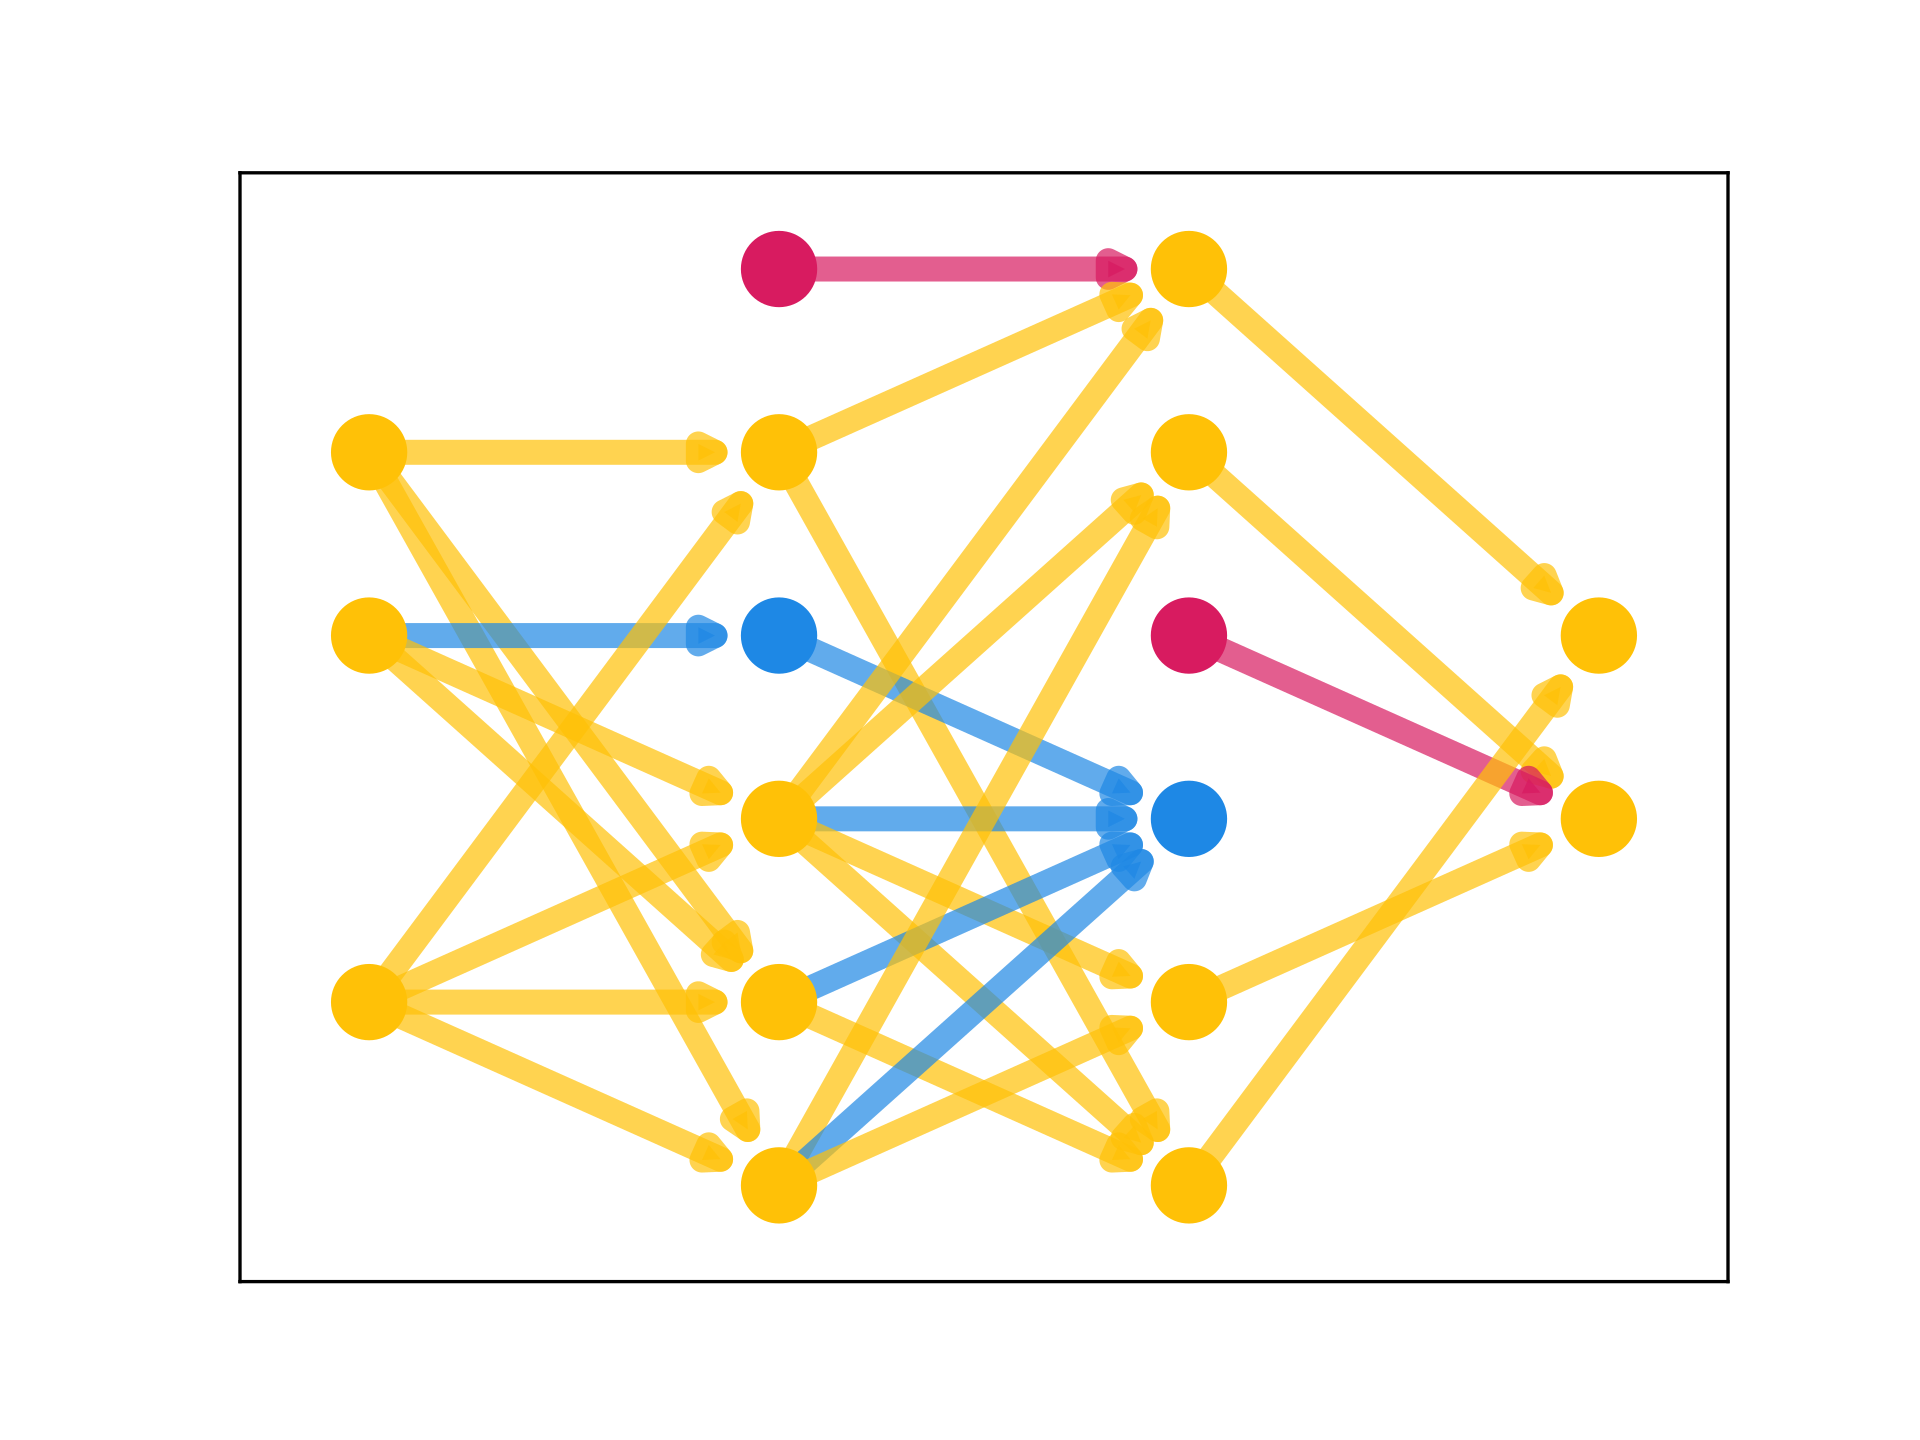
\includegraphics[width=.5\linewidth]{active-example.png}
    \caption[Active, inactive and zombies example]{
    A sample network with active (yellow), inactive (blue) and zombie (magenta) parameters.
    }\label{fig:parameter_categories}
\end{figure}

In figure~\ref{fig:parameter_categories}, the different categories are visualized.
The network input is on the left and the output is on the right.
In magenta, the zombie parameters which are not connected to any input are shown.
In blue, inactive parameters that are not connected to any output are shown.
The rest of the network consists of active parameters in yellow, which are connected to both input and output.
Pruned parameters are not actively visualized, since they are removed from the network.

\subsection{Finding Subnetworks}\label{sec:FindSubnet}
To find independent subnetworks in the network, the previously defined categories are assigned to each parameter after every pruning level.
First, after a network is pruned, each newly pruned weight is categorized as such.
From the directed acyclic graph of the network $\mathcal{G}$ that contains the parameters of all categories a subgraph is created.
Concretely, let $\mathcal{G}$ be defined as the pair $\{V, E\}$, where $V$ is the set of all vertices or nodes and $E$ is the set of all edges.
The set $E_p$ is a subset of $E$, containing all pruned edges of the graph.
The set of unpruned edges $E_{\neg p}$ is defined as:
\[ E_{\neg p} = E - E_p \]
, where $E-E_p$ denotes the set difference.
Since biases are not pruned, the set of unpruned nodes is simply $V_{\neg p} = V$
With the vertices $V_{\neg p}$ and the unpruned edges $E_{\neg p}$ a subgraph of $\mathcal{G}$ is created, denoted $\mathcal{G}_{\neg p}$.

On this subgraph, $\mathcal{G}_{\neg p}$, inactive nodes and edges are found and assigned their category.
To find inactive parameters, each node except the output nodes is examined.
A node is inactive, if it does not have a valid path to any of the output neurons.
Since the graph is directed, the path is only allowed along the direction of the edge.
Consequently, all incoming edges of an inactive node are also inactive.

The set $E_i$ is a subset of $E_{\neg p}$, and it contains all the inactive edges.
Similarly, the set $V_i$ is a subset of $V_{\neg p}$ and contains all the inactive nodes.
All nodes and edges that are neither pruned nor inactive are collected in the sets $V_{\neg pi}$ and $E_{\neg pi}$ respectively.
They are defined as:
\[ V_{\neg pi} = V_{\neg p} - V_i \]
\[ E_{\neg pi} = E_{\neg p} - E_i \]

The subgraph of $\mathcal{G}_{\neg p}$, which contains only the nodes in $V_{\neg pi}$ and the edges in $E_{\neg pi}$ is denoted $\mathcal{G}_{\neg pi}$.

On the subgraph $\mathcal{G}_{\neg pi}$, which neither contains pruned nor inactive parameters, all zombie parameters are collected.
All nodes, where there is no path from any input to the node, are collected in the set $V_z$.
Further, all edges to or from nodes in the set $V_z$ are collected in $E_z$.
The sets of the remaining active nodes and edges are defined as:
\[ V_a = V_{\neg piz} = V_{\neg pi} - V_z \]
\[ E_a = E_{\neg piz} = E_{\neg pi} - E_z \]
Because all categories of parameters except for active ones are removed from the sets, they are simply denoted $E_a$ and $V_a$ for short.

With the sets $V_a$ and $E_a$, a new subgraph is created, that represents the active part of the graph $\mathcal{G}$, called $\mathcal{G}_a$.
This active subgraph $\mathcal{G}_a$ is further used to find separated components of the network.

\begin{figure}[ht] % find connected components
\centering
\begin{minipage}{\linewidth}
\begin{lstlisting}[
    language=Python,
    captionpos=b, 
    label={code:split},
    caption={[Finding independent subnetworks]
    Finding independent subnetworks in a neural network with PyTorch~\autocite{networkx} and networkx~\autocite{networkx}; Python pseudo code
    },
]
import torch
import networkx as nx

model: torch.nn.module  #  the neural network

# torch model -> networkx directed acyclic graph
G: nx.DiGraph = transform_to_digraph(model)

# remove pruned, inactive, and zombie parameters
G_not_p = remove_pruned_parameters(G)
G_not_pi = remove_inactive_parameters(G_not_p)
G_a = G_not_piz = remove_zombie_parameters(G_not_pi)

# check for independent subgraphs in the active graph
subnetworks = []
for c in nx.connected_components(G_a.to_undirected()):
    subnetwork = G_a.subgraph(c)
    subnetworks.append(subnetwork)
\end{lstlisting}
\end{minipage}
\end{figure}

The code snippet~\ref{code:split} outlines the process of finding the subnetworks.
A neural network first is converted into a directed acyclic graph.
The network is implemented with PyTorch~\autocite{pytorch}, a commonly used machine learning library and converted into a graph which is further processed with NetworkX~\autocite{networkx}, a well-known library for working with mathematical graphs.
As described previously, the active subgraph \lstinline{G_a} is created.
Connected components of the graph, if there are more than one, are obtained.
A connected component is a subgraph of a graph, where every node is connected via a path to every other node.
Therefore, if the graph is separated, there exist at least two connected components.
The function \lstinline{nx.connected_components}, provided by NetworkX, retrieves all the connected components.

\section{Datasets with Independent Tasks}\label{sec:taskmatch}
In this thesis, one area of interest is to see if the network separates given that there exist independent tasks in the dataset.
Critically, it is important to know if the network separates such that it is connected to one task but not the other.
This section explains how the connected components obtained via the methods described in section~\ref{sec:FindSubnet} are then matched to the tasks of the dataset.

\subsection{Definition of Tasks in Datasets}
Consider the dataset $\mathcal{D}$ with its set of input features $\mathcal{D}_X$ and output features or labels $\mathcal{D}_Y$.
Let $T$ be a task, which is defined by the inputs $T_X$ and outputs $T_Y$ that belong to the task, where $T_X$ is a subset of $\mathcal{D}_X$ and $T_Y$ a subset of $\mathcal{D}_Y$.
The tasks $T$ is said to be independent if the set of inputs $T_X$ and outputs $T_Y$ are not shared with any other task.
Independent tasks must not overlap.
Classical machine learning datasets like MNIST~\autocite{mnist} contain one independent task because all input features may be necessary to predict all labels.

However, there can exist datasets with more than one independent task.
Concretely, consider a task $T^{(1)}$ with inputs $T^{(1)}_X$ and outputs $T^{(1)}_Y$ and task $T^{(2)}$ with inputs $T^{(2)}_X$ and outputs $T^{(2)}_Y$.
The sets of inputs $T^{(1)}_X$ and $T^{(2)}_X$ are both subsets of $\mathcal{D}_X$, but are disjoint $T^{(1)}_X \cap T^{(2)}_X = \emptyset$.
The same is true for the input sets.
The set $T^{(1)}_X$ contains information that is relevant to compute the outputs $T^{(1)}_Y$, but no helpful information to compute $T^{(2)}_Y$.
Similarly, the set $T^{(2)}_X$ does not contain information that is useful to compute $T^{(1)}_Y$.
To be able to match networks with tasks, the inputs and outputs of the tasks must be defined alongside the dataset.
Datasets that contain two independent tasks will be created in chapter~\ref{chapter:experiments}.

\subsection{Matching Subnetworks with Tasks}
The subnetworks that are found with the methods described in section~\ref{sec:FindSubnet} now must be matched with the tasks.
For each subnetwork and each task in the dataset, the inputs and outputs of the network are compared to the inputs and labels of the task.

Let $T^{(i)}$ be an independent task that has associated input features in the set $T^{(i)}_X$ and the output features in $T^{(i)}_Y$.
Further, the input and output neurons of a network $j$ are referred to as $N^{(j)}_X$ and $N^{(j)}_Y$ respectively.
For each network and each task, the amount to which the network covers the inputs or outputs of the task can be calculated.
Regarding the inputs, this quantity $c^{(i)}_X$ is referred to as input-coverage. The output-coverage is denoted as $c^{(i)}_Y$.

The number of features that are covered by the network is calculated as the cardinality of the intersection of the network features and the task features $ |N \cap T|$, where  $|A|$ denotes the cardinality of set $A$.
To attain the coverage, the number of features covered by the network is divided by the number of features the task contains.
Then, the coverage is calculated for inputs and outputs as 

\[
c^{(i)}_X = \frac{|N^{(j)}_X  \cap T^{(i)}_X |}{|T^{(i)}_X|} \quad\textit{,where}\quad 0 \leq c^{(i)}_{X} \leq 1\
\]
\[
c^{(i)}_Y = \frac{|N^{(j)}_Y  \cap T^{(i)}_Y |}{|T^{(i)}_Y|} \quad\textit{,where}\quad 0 \leq c^{(i)}_{Y} \leq 1\
\]
Both coverage terms evaluate to $1$ if the network covers all the inputs or outputs of the task.
If the network does not cover any of the inputs or outputs, the input- or output coverage evaluates to $0$ respectively.
The total coverage $c^{(i)}_{XY}$ of the task can be calculated as the product of the input and output coverage.
\[ c^{(i)}_{XY} = c^{(i)}_{X} * c^{(i)}_{Y} \quad\textit{,where}\quad 0 \leq c^{(i)}_{XY} \leq 1\]
The value of the total coverage evaluates to $1$ if both input and outputs are completely covered.
It evaluates to $0$, as soon as either the inputs or outputs are not covered at all.
Depending on the dataset, either of the coverage terms might be used to assess the extent to which the network matches the task.
Consider a scenario where all the inputs and outputs of the task are strictly necessary for the network to perform properly.
Then, the total coverage is a valuable measure.
In a scenario where all outputs are necessary to perform, but not all inputs are important, the output-coverage might be the better measure.

\subsection{Separation, Degradation and Interconnectedness}
Now with the coverages calculated, the network can be categorized.
First, a coverage term that is used for the categorization must be selected.
Consider the network $N$ with $J$ subnetworks $\{N_1, \dots, N_J\}$ and a dataset $\mathcal{D}$ with $K$ tasks $\{T_1, \dots, N_K\}$.
Either the input-, output- or total coverage can be used and will be referred to as $c^{(k)}$ for task $k$ in this section.

The network $N$ is assigned to one of three categories, depending on the coverage of its subnetworks:
\begin{itemize}
    \item \textbf{Interconnected}: The network is considered interconnected if the coverage of each task is $1$, but the networks are not separated. Therefore, the number of tasks $K$ is greater than the number of subnetworks $J$.
    An unpruned, fully-connected network is per definition interconnected.
    \[ c^{(k)} = 1; \quad\forall\quad k \in [1, \dots, K]\]
    \[ K > J \]

    \item \textbf{Separated}: The network is considered separated if the coverage of each task is $1$, and there is an equal number of subnetworks and tasks.
    \[ c^{(k)} = 1; \quad\forall\quad k \in [1, \dots, K]\]
    \[ K = J \]

    \item \textbf{Degraded}: The network is considered degraded if the coverage of at least one task is less than $1$.
    \[ c^{(k)} < 1; \quad\textit{for any}\quad k \in [1, \dots, K]\]
\end{itemize}

Concretely, consider a dataset that contains two tasks, $T^{(1)}$ and $T^{(2)}$, with their accociated input sets $T^{(1)}_X$, $T^{(2)}_X$ and output sets $T^{(1)}_Y$, $T^{(2)}_Y$.
Let $J$ denote the number of subnetworks.
The coverages can be collected in a matrix $C$ of size $J \times K$, where $K=2$. 
$c_{j,k}$ represents the value at the $j$-th row and the $k$-th column and $0 \leq c_{j,k} \leq 1$ holds.
The sum of the matrix is upper bound by the number of tasks $K$.
\[ \sum_{j=1}^{J} \sum_{k=1}^{K} c_{j,k} \leq K \]
Given an unpruned network and a dataset with two tasks the matrix would look like the following 
\[ C = \begin{pmatrix} 1 & 1 \end{pmatrix} \]
Each task would be completely covered by the same network.
Since the network per definition covers all tasks before the first pruning level, the matrix will be a unit vector with as many entries as there are tasks.
This network is \textbf{interconnected}.

After several pruning iterations, the network might contain two disconnected subnetworks.
In this case, an additional row is added to the matrix.
For instance, let the subnetworks perfectly match the tasks such that every task is completely covered by one subnetwork.
This network is considered \textbf{separated} and the matrix $C$ might look like the following.
\[ C = \begin{pmatrix} 1 & 0 \\ 0 & 1 \end{pmatrix} \]

After the network is pruned further, all the connections to one of the input nodes might be pruned.
Then, one of the subnetworks would not be completely covered anymore.
This network is considered \textbf{degraded}.
Assuming that half of the features of interest of a given task are not covered anymore, the resulting matrix $C$ would look like the following.
\[ C = \begin{pmatrix} 1 & 0 \\ 0 & 0.5 \end{pmatrix} \]

If the sum of $C$ is equal to the number of tasks and the number of subnetworks is equal to the number of tasks, then the network is (perfectly) separated.
If the sum of $C$ is equal to the number of tasks, but there are fewer subnetworks than tasks, the network still needs to separate.
The number of separations that are required can be calculated by the difference between the number of tasks and the number of subnetworks.
If the sum of $C$ is less than the number of tasks, the network already has lost at least one input or output.
This scenario is referred to as a degraded network.
Once a network is degraded, a perfect separation cannot be reached anymore.
Generally, throughout this thesis, the training is stopped as soon as the network is degraded to save computational resources.

\chapter{Experiments and Results}\label{chapter:experiments} 
In this chapter, an empirical investigation into the structure of winning tickets is conducted.
First, the datasets that were used are described in detail.
Then, experiments were conducted that attempt to find separate subnetworks in the winning ticket, for both datasets.
Finally, the connectivity of the network to the network input is examined.

\section{Datasets}
\textcite{BIMT} conducted experiments on symbolic regression datasets.
These are simple toy datasets where the labels are computed with a symbolic formula. 
For instance regarding the independence task, the inputs are $x_1, x_2, x_3, x_4$ and the outputs are $y_1={x_2}^2 + \sin{(\pi*x_4)}$ and $y_2={(x_1+x_3)}^3$.
In this case, the independence is obvious, as $y_1$ depends only on $x_2$ and $x_4$, and $y_2$ depends only on $x_1$ and $x_3$.
However, concerning the lottery ticket hypothesis, the existing literature focuses on classification tasks, while this is a regression task.
Therefore instead of using the independence dataset from \textcite{BIMT}, 
two classification datasets that contain independent tasks are created in the scope of this thesis, which are described in the following sections.

\subsection{Moons-Circles Dataset}\label{sec:independece_dataset}
The first dataset is a combination of two classic toy datasets, which are concatenated into one dataset.
The two selected datasets are the Two-Moons dataset and the Circles dataset, depicted in figure~\ref{fig:moons_circles}.
Both datasets can be interpreted as a two-dimensional plane, where the inputs describe the coordinates of points on the plane. 
The labels of the dataset relate to the class, either red or blue.

\begin{figure}
\centering 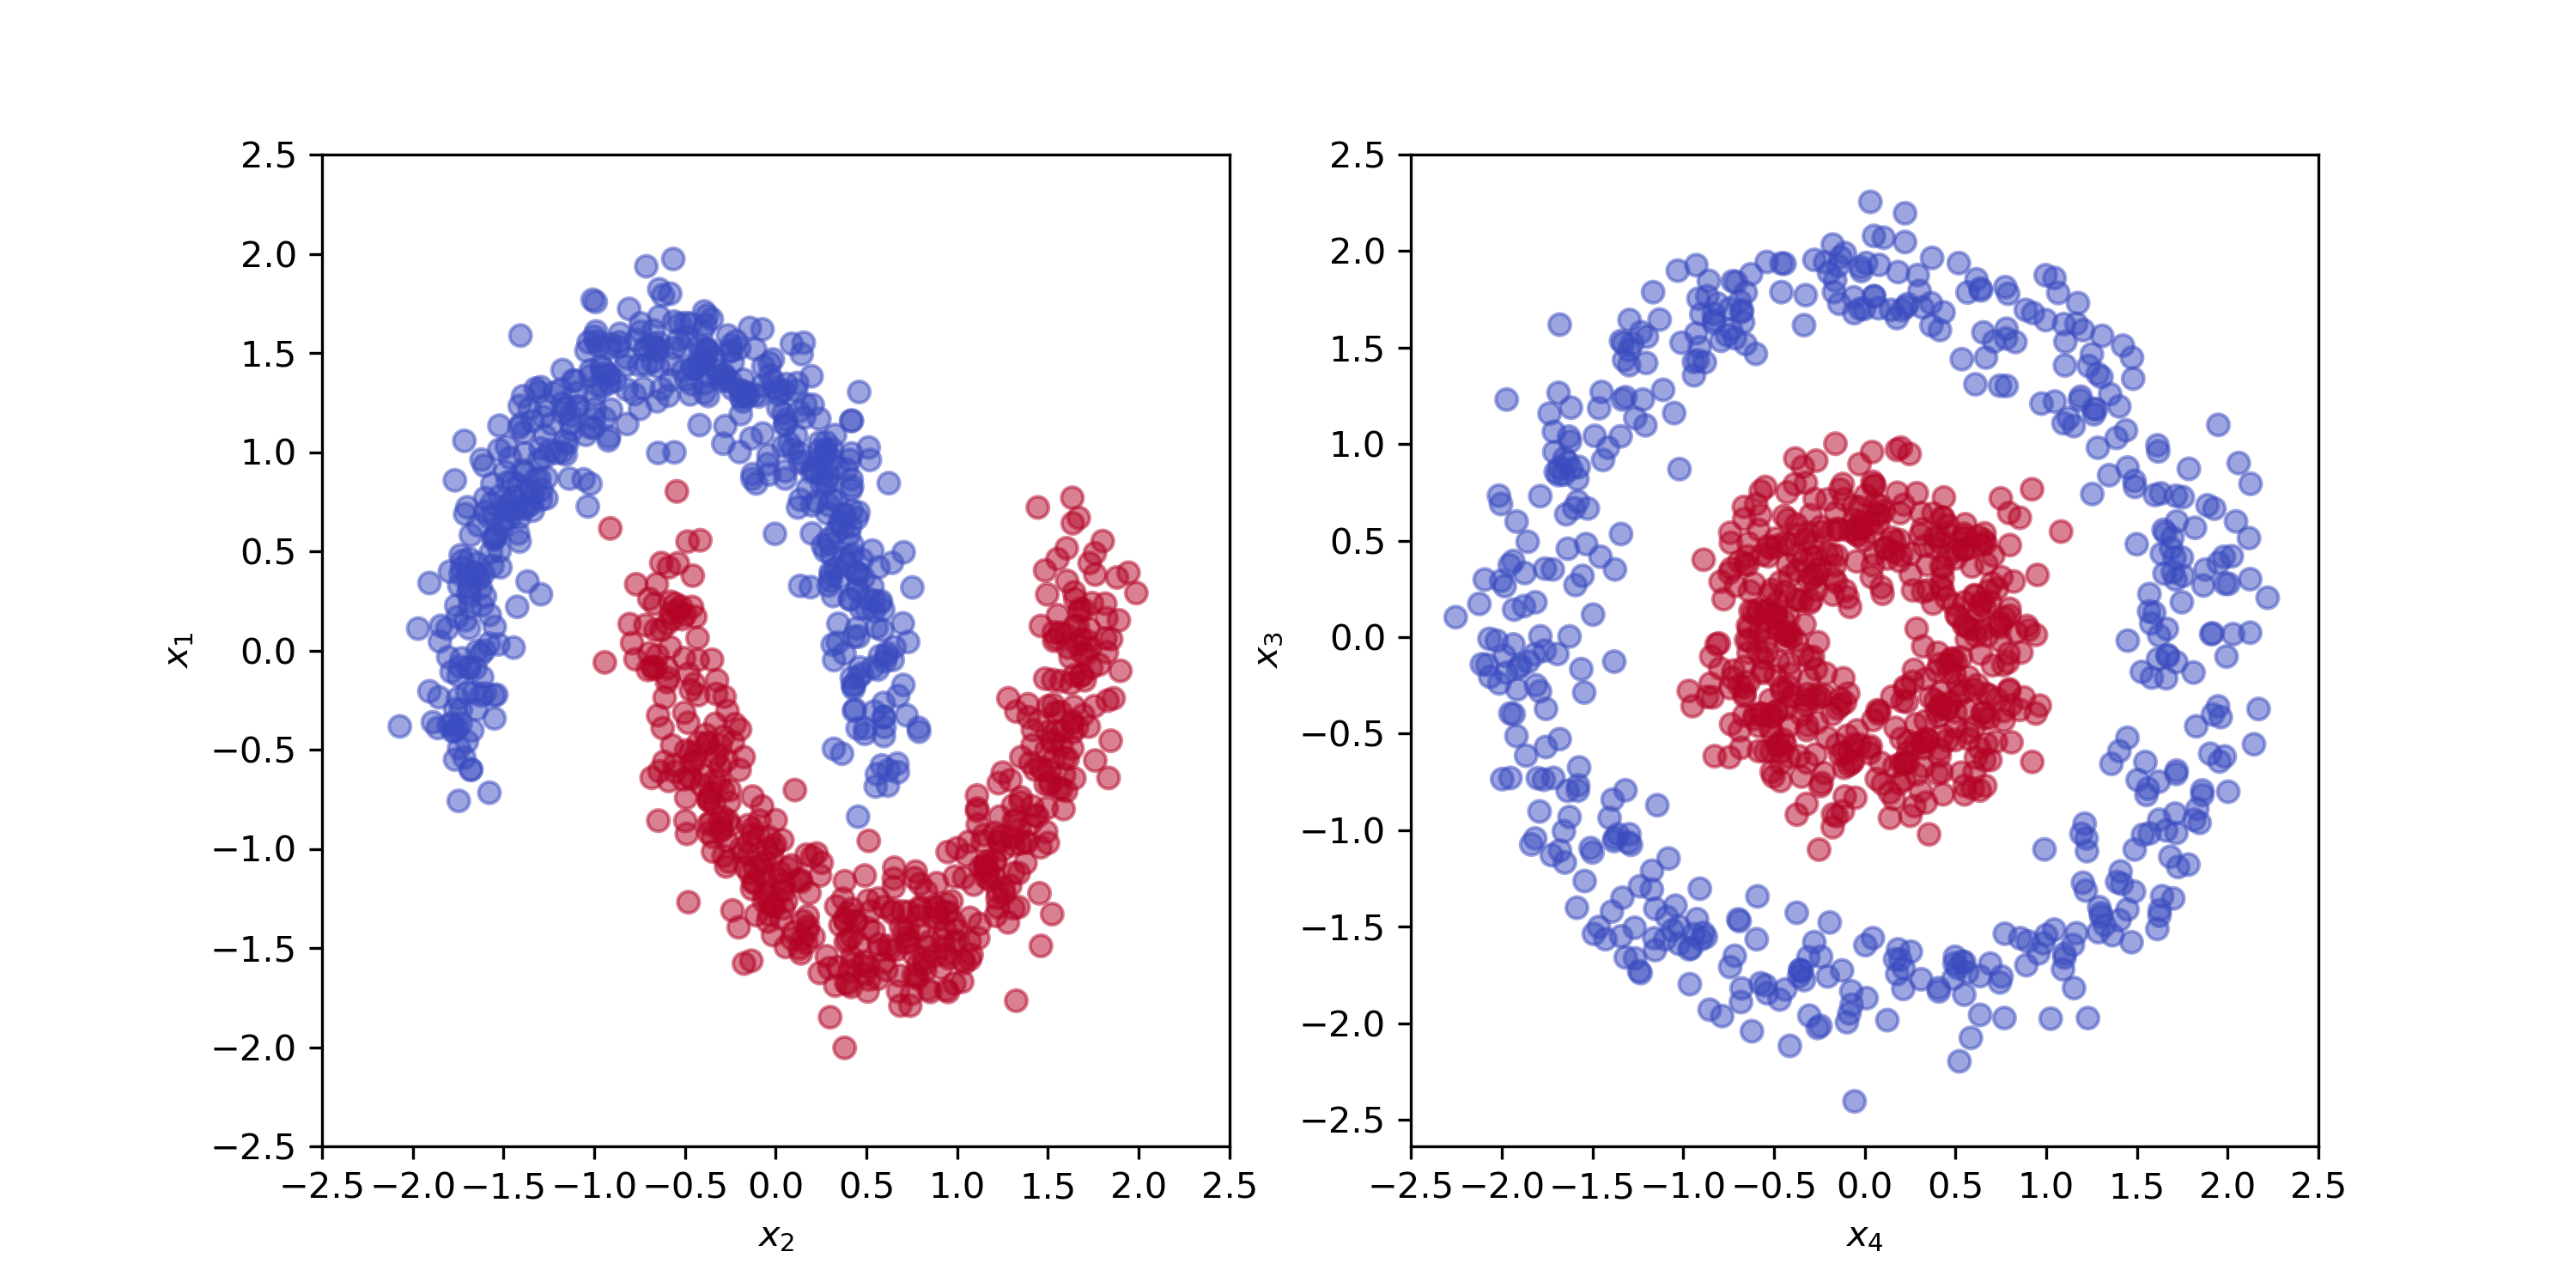
\includegraphics[width=1.0\linewidth]{moons-circles.png}
\caption[Two-Moons and Circles Dataset]{
    The Two-Moons dataset (left) and the Circles dataset (right); normalized to zero mean and unit variance.}\label{fig:moons_circles}
\end{figure}

Concretley, let $( x_1 , x_2 )$ be the inputs of the Two-Moons dataset and $y_1 \in \{0,1\}$ the class label.
The samples are generated by creating two half circles of evenly spaced points, with a radius of one.
One of the half circles is rotated by 180 degrees and shifted by $0.5$.
Gaussian noise with a mean of zero and standard deviation of $0.1$ is added to each point in the dataset.
Let $( x_3 , x_4 )$ be the inputs of the cirlces dataset and $y_2 \in \{0,1\}$ the class label.
The data is generated by creating evenly spaced points on the inner and outer circles. 
The center of both circles is at $(0,0)$ and the radius of the outer circle is one.
The radius of the inner circle is set to be $0.35$.
Gaussian noise with a mean of zero and standard deviation of $0.1$ is added to each point in the dataset.
The values of noise and the size of the inner circle are selected, such that the points do not mix among the circles.

\begin{figure}[t]
\centering
\begin{minipage}{\linewidth}
\begin{lstlisting}[
    language=Python,
    captionpos=b, 
    label={code:data},
    caption={[Dataset Generation]Generation of Moons-Circles dataset with scikit-learn~\autocite{sklearn}; pseudo code},
]
from sklearn import make_circles, make_moons
from sklearn.model_selection import train_test_split

# generates shuffled data points with labels
# x1, x2 -> shape=(1000, 2); y1, y2 -> shape=(1000, ) 
x1, y1 = make_circles(n_samples=2000, noise=0.1, factor=0.35)
x2, y2 = make_moons(n_samples=2000, noise=0.1)

circles_moons_x = concatenate(x1, x2) # shape=(1000,4)
circles_moons_y = concatenate(y1, y2) # shape=(1000,2)

# split the dataset in half
x_train, x_test, y_train, y_test = train_test_split(
    circles_moons_x, circles_moons_y, test_size=0.5
)

# scale data to zero mean, unit variance, based on training data
scaler = sklearn.preprocessing.StandardScaler().fit(x_train)
x_train = scaler.transform(x_train)
x_test = scaler.transform(x_test)

(x_train, y_train) # the training data
(x_test, y_test) # the test data
\end{lstlisting}
\end{minipage}
\end{figure}

The classic machine learning library Scikit-Learn~\autocite{sklearn} is used to generate the data. 
The code snippet~\ref{code:data} outlines the generation process as Python-flavoured pseudo code.
The previously described sampling strategies for the data relate to the implementation in the Scikit-Learn Python library.
The data is generated with the \lstinline{makemoons}, and \lstinline{makecircles} functions, respectively.
Since the ranges of values of the datasets are different due to their sampling strategy, each feature is normalized individually to have zero mean and unit variance.
The final, normalized datasets are depicted in figure~\ref{fig:moons_circles}

To create a single dataset out of the two separate datasets, the input features as well as the labels are concatenated.
Concretely, one sample of the concatenated dataset $\hat x$ contains one randomly selected sample from the Two-Moons dataset and one randomly selected sample from the Circles dataset.
The label $\hat y$ of the sample $\hat x$ also consists of the respective concatenated labels.
\[\hat x = ( x_1 , x_2 , x_3 , x_4 )\]
\[\hat y = ( y_1 , y_2 )\]
In this way, the whole dataset is concatenated.
Afterward, the dataset is randomly split in half into a training set and a test set.
The result is a training set and a test set with 1000 samples each.
This dataset contains two separate and independent tasks.
For each task, only the respective inputs contain valuable information for the prediction of the class.

\begin{figure}[t]
    \centering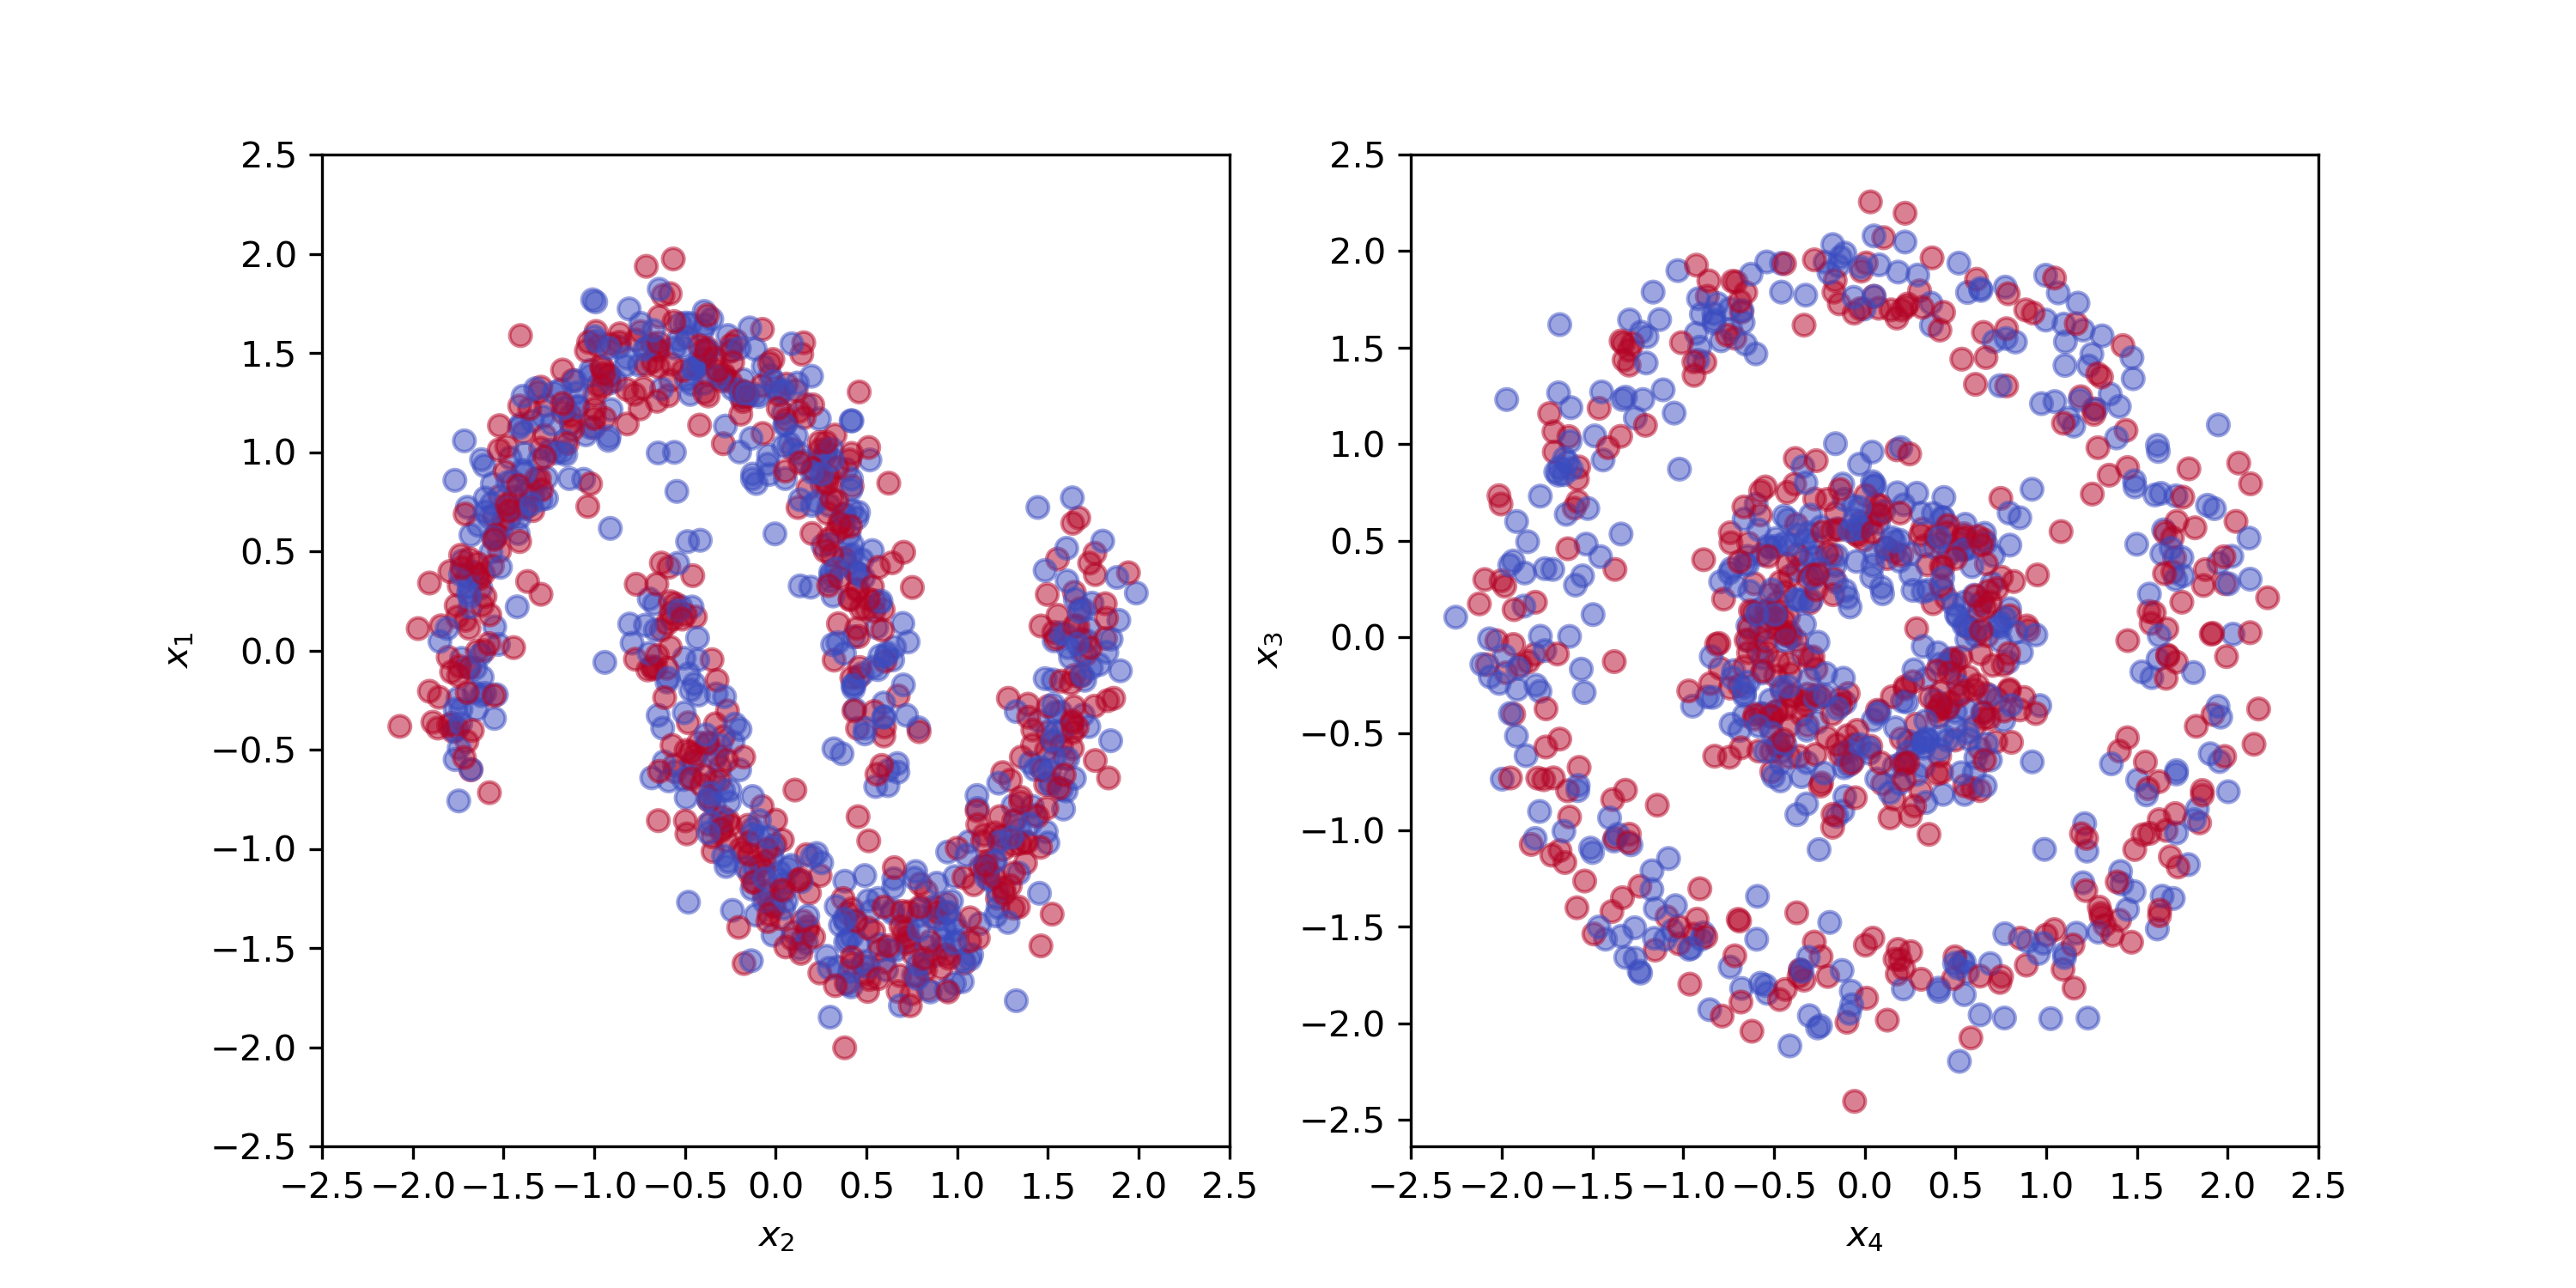
\includegraphics[width=1.0\linewidth]{moons-circles-inverted.png}
    \caption[Two-Moons and Circles Dataset, inverted labels]{
        The Two-Moons dataset (left) with Circles labels, and the Circles dataset (right) with Two-Moons labels. 
    }\label{fig:moons_circles_inverted}
\end{figure}

The independence is demonstrated in figure~\ref{fig:moons_circles_inverted}.
The dataset is the same as is visible in figure~\ref{fig:moons_circles}. 
However, the Two-Moons dataset is displayed with the labels of the Circles dataset and vice versa.
Concretely, on the left side, the coordinates represent $x_1$ and $x_2$, but the colors refer to $y_2$.
On the right side on the other hand, $x_3$ and $x4$ are displayed with the colors defined by $y_1$.
There is no clear visible pattern discernible from these datasets given on their own.

The generation procedure of the datasets is outlined in the Python-flavoured pseudo code snippet~\ref{code:data}.
First, both datasets are individually generated.
The samples and labels are then concatenated into one dataset, which is then randomly split into the training and test set.
Finally, the data is normalized to zero mean and unit variance, based on the training set.
The generated dataset will be referred to as the \textit{Moons-Circles} dataset.

\subsection{MNIST-Fashion-MNIST Dataset}\label{sec:mnist}
To test the network separation on a slightly more realistic problem, the MNIST-Fashion-MNIST dataset is created.
The dataset is created similarly to the Moons-Circles dataset described in paragraph~\ref{sec:independece_dataset}, but the MNIST dataset~\autocite{mnist} and the Fashion-MNIST~\autocite{fashion} dataset are used as tasks.
The MNIST dataset is a well-known dataset of handwritten digits. 
The training set consists of 60000 images and the test set of 10000.
It contains all digits from zero to nine in handwritten form, on a $28 \times 28$ pixel grayscale image.
This dataset was also used in the original lottery ticket experiments by~\textcite{LTH}.

\begin{figure}[t]
    \centering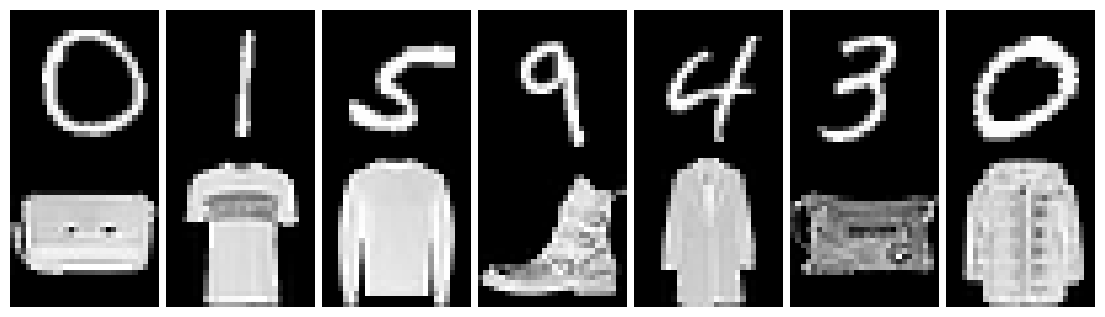
\includegraphics[width=1.0\linewidth]{mnist-fashion-mnist.png}
    \caption[MNIST-Fashion-MNIST dataset]{
        The MNIST-Fashion-MNIST dataset; Each sample contains a random MNIST image (top) and a random Fashion-MNIST image (bottom).
    }\label{fig:mnist_fashion}
\end{figure}

As the name suggests, the Fashion-MNIST dataset~\autocite{fashion} is similar to the MNIST dataset.
However, instead of handwritten digits, different items of clothing are displayed on the $28 \times 28$ grayscale image.
It contains the same number of images for the test set and the training set.
Both datasets contain 10 classes.
In the same way as described in paragraph~\ref{sec:independece_dataset}, the datasets are concatenated into one.
Both datasets are shuffled and each sample from the MNIST dataset is concatenated with a random sample from the Fashion-MNIST dataset.
The class labels are also concatenated.
The result is a dataset with 60000 training samples and 10000 evaluation samples.
Through the concatenation, each image has an aspect ratio of $28 \times 56$, where each half corresponds to one of the datasets.
In figure~\ref{fig:mnist_fashion}, seven randomly selected samples of the  MNIST-Fashion-MNIST dataset are displayed.
On the top of each image, the handwritten MNIST digit is displayed. 
On the bottom the fashion item is visible.
Each sample consists of one random digit and one random fashion item. 

Contrary to the previous task, this dataset contains significantly more input features.
Each dataset has 784 input features, which results in 1586 input features for the concatenated dataset.
The Moons-Circles dataset only has four input features and two output features.
Further, the previous task was a combination of two binary classification tasks.
Now, each dataset represents a multiclass classification problem with 10 classes.

\newpage
\section{Experiments on the Moons-Circles Dataset}
The first round of experiments is dedicated to finding out what conditions are required, such that the network separates when trained on the Moons-Circles dataset.
During a preliminary exploration phase, some scenarios where the network indeed separates were found.
Yet, they were sparse and could not be easily interpreted.
Therefore, in this step, the knowledge gained from the initial experiments was put to use.
A systematic evaluation of the relationship between network size and splitting behavior was conducted.

To enable comparison between networks of different sizes, the network extension technique described in paragraph~\ref{sec:extension} was used.
First, an extensive experiment with a base network architecture of $(4,8,8,2)$ was conducted.
To expand the range of the results, two additional experiments were conducted, which were slightly smaller to lower computational cost.
One experiment is done on a network with only one hidden layer, concretely with a shape $(4,20,2)$, and the other experiment on a network with three hidden layers, a shape of $(4,4,4,4,2)$.
All other hyperparameters are shared among the three experiments.
The only difference is the pruning target, which is derived from the network architecture.

For all three experiments, the pruning rate was set to $0.32$.
The chosen value, while somewhat arbitrary, was selected by promising results on preliminary tests.
\textcite{LTH} used a pruning rate of $0.2$ in the original experiments for the fully connected feed-forward network trained on the MNIST dataset.
However, with a larger pruning rate, a larger space of network sizes can be covered with the same number of iterations, which is why the larger pruning rate of $0.32$ was selected.

\subsection{Exploring Network Architectures - Model Extension}\label{two-hidden}
The first experiment architecture that is discussed is the network with two hidden layers.
The base network, which is the network that is used as a base for extending, has the shape $(4,8,8,2)$.
This architecture has 112 weights, which is also used as the pruning target.
The network architecture indicated by the number of neurons per hidden layer and the respective number of weights are displayed in table~\ref{tab:trajectory}.
The network is extended up to 25 times.
At the extension level 25, the network has a shape of $(4,1310,1310,2)$, with 1.723.960 weights.
The number of extension levels corresponds to the number of pruning levels the network goes through.
After each pruning level, the network is evaluated to check if it is separated or degraded.

When considering all pruning levels, there are four different scenarios for a network:
\begin{enumerate}
\item \textbf{Separated:}
The network separates at some pruning level. 
It does not degrade at any later level. 
\item \textbf{Separated-Degraded:} 
The network splits at some point and has all input and output nodes.
At a later level, the network degrades (it loses at least one input or output).
\item \textbf{Degraded:} 
The network degrades before it can separate.
\item \textbf{Interconnected:} 
The network does neither separate nor degrade. 
The result is a single network that contains all input and output nodes of all tasks.
\end{enumerate}

\begin{table}[t]\scriptsize
    {
    \sffamily
    \caption[Parameter Trajectories of different network sizes]{
    In this table, the parameter trajectories and the corresponding hidden dimension of the network are displayed for each extension level. 
    The parameter trajectory is in each respective `param' column and the number of hidden neurons per hidden layer is in the column `hidden'.
    At the extension level zero, the base model values are displayed.
    }\label{tab:trajectory}
    \begin{tabular}{rrrrrrr}
    \toprule
    Lvl & hidden-1 & param-1 & hidden-2 & param-2 & hidden-3 & param-3 \\
    \midrule
    0 & 20 & 120 & 8 & 112 & 6 & 108 \\
    1 & 29 & 174 & 10 & 160 & 8 & 176 \\
    2 & 43 & 258 & 13 & 247 & 10 & 260 \\
    3 & 64 & 384 & 16 & 352 & 12 & 360 \\
    4 & 94 & 564 & 20 & 520 & 15 & 540 \\
    5 & 138 & 828 & 25 & 775 & 19 & 836 \\
    6 & 202 & 1212 & 31 & 1147 & 23 & 1196 \\
    7 & 297 & 1782 & 38 & 1672 & 29 & 1856 \\
    8 & 437 & 2622 & 47 & 2491 & 35 & 2660 \\
    9 & 643 & 3858 & 57 & 3591 & 43 & 3956 \\
    10 & 946 & 5676 & 70 & 5320 & 52 & 5720 \\
    11 & 1391 & 8346 & 85 & 7735 & 63 & 8316 \\
    12 & 2046 & 12276 & 104 & 11440 & 77 & 12320 \\
    13 & 3009 & 18054 & 127 & 16891 & 94 & 18236 \\
    14 & 4425 & 26550 & 154 & 24640 & 114 & 26676 \\
    15 & 6507 & 39042 & 188 & 36472 & 139 & 39476 \\
    16 & 9569 & 57414 & 229 & 53815 & 169 & 58136 \\
    17 &   &   & 278 & 78952 &   &   \\
    18 &   &   & 337 & 115591 &   &   \\
    19 &   &   & 410 & 170560 &   &   \\
    20 &   &   & 498 & 250992 &   &   \\
    21 &   &   & 604 & 368440 &   &   \\
    22 &   &   & 733 & 541687 &   &   \\
    23 &   &   & 890 & 797440 &   &   \\
    24 &   &   & 1080 & 1172880 &   &   \\
    25 &   &   & 1310 & 1723960 &   &   \\
    \bottomrule
    \end{tabular}
    }
\end{table}

\begin{figure}[t] % Stacked Area d=2
    \centering
    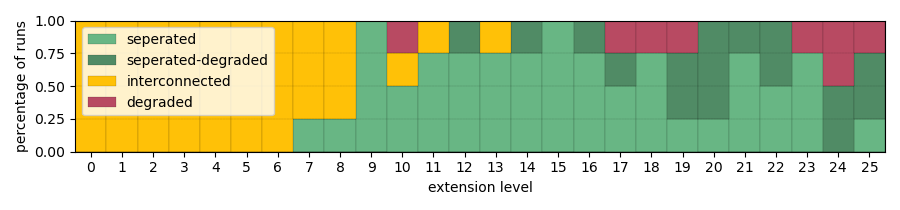
\includegraphics[width=1.0\linewidth]{2-layer-histogram-split-behaviour.png}
    \caption[Separation/Degradation Stacked Area Chart (2 hidden layers)]{
        A proportional stacked area chart showing the ratio of training runs in each category.
        The x-axis shows the extension level, and the y-axis shows the relative amount of networks in each category, stacked. (2 hidden layers)
        }\label{fig:2laxer-histogram}
\end{figure}

At each extension level, the runs are repeated with four different seeds for the network initialization.
The results are displayed in figure~\ref{fig:2laxer-histogram}.
The figure is a proportional stacked area chart, where each scenario described above is encoded with a color.
On the x-axis, the extension levels are shown.
On the y-axis, the percentage of networks in each category can be viewed.
A clear pattern in the data is, that the networks separate for the first time with at least 7 pruning levels.
The shape and number of weights at that level are $(4,38,38,2)$ and 1672 respectively, which is $\sim15$ times the number of weights compared to the base model. 
Starting at shape $(4,57,57,2)$ or extension level 9, which represents an increase of $\sim32$-times, the majority of the networks separate.
Up until the 6th extension level, none of the networks separate or degrade. 
However, if the network were pruned further, at some point every network would degrade eventually.
Therefore it is also reasonable to assume that some of the networks that are still interconnected after all pruning iterations would separate if they were pruned to a lower pruning target.

Another interesting observation is that only after extension level 10 the networks begin to degrade.
What follows from the data is the more extension levels, the more likely it is that a network degrades, either before or after it separates.
One possible explanation for this is that at each pruning level, a certain number of weights are made inactive.
As noted in \autocite{HanEtAl15, AllAlivePruning}, this is a known phenomenon.
However, since no regularization is used in these experiments, the inactive weights do not decrease in magnitude.
Rather, they are frozen with their last value.
If more inactive parameters are created at each pruning level than pruned, the percentage of inactive weights in the network grows with every iteration.
Therefore, the more pruning levels the network experienced, the less of its available, unpruned parameters are active.
This effectively makes the network smaller, which in turn makes it more likely to separate or degrade.

\begin{figure}[ht] % Less active more pruning
    \centering
    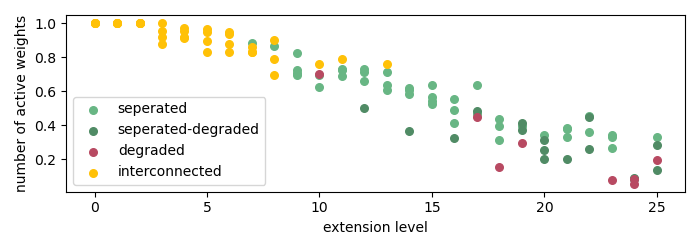
\includegraphics[width=1.0\linewidth]{2-layer-compund-damage.png}
    \caption[Correlation extension levels and rate of active weights]{
    The correlation between the number of extension levels and the percentage of active weights in the network.
    Each dot is a single training run, the colors indicate the category of the training run. (2 hidden layers)
    }\label{fig:collateral_damage}
\end{figure}

This effect is visualized in figure~\ref{fig:collateral_damage}.
The colors are encoded in the same way as in figure~\ref{fig:2laxer-histogram}.
Each dot represents a single training run. 
On the x-axis, the extension level is displayed.
On the y-axis, the number of active weights after the last pruning level is displayed.
A clear pattern emerges, showing a correlation between the number of pruning iterations and the number of active weights in the final network.
Important to note is that when a network degrades (red), the run is immediately stopped.
Therefore in this graph, the degraded networks might have larger numbers of active weights, compared to other networks that were pruned for the total amount of levels.
However, even with this caveat, a clear trend is visible.
The more pruning levels the network experiences, the smaller the percentage of the active network weights.
For some networks that were extended to 20 or more levels, the final percentage of active weights in the network is only $\sim20$ percent, which translates to only $\sim22$ active weights.
Techniques like L1-Regularisation used in \autocite{HanEtAl15} or All-Alive-Pruning \autocite{AllAlivePruning} could counteract this effect of compounding inactive parameters.
However, this is a topic for future research and is not addressed further in this thesis. 

To gain a broader picture of the effects shown on the network with two hidden layers, the same experiments were conducted on networks with one and three hidden layers.
Similar effects can be seen for these architectures.
As shown in table~\ref{tab:trajectory}, the networks were only extended for 16 levels instead of 25, to reduce computational requirements. 
As the networks get larger and the number of pruning levels is higher, the computational effort increases significantly.
For the network with one hidden layer a base network with shape $(4,20,2)$ was selected.
It has a similar number of weights compared to the base network with two layers.
\begin{figure}[t] % Stacked Area d=1
    \centering
    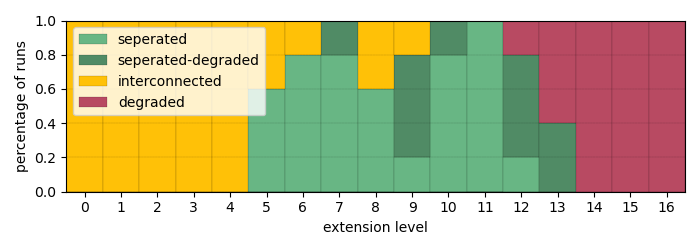
\includegraphics[width=1.0\linewidth]{1-layer-histogram-split-behaviour.png}
    \caption[Separation/Degradation Stacked Area Chart (1 hidden layer)]{       
        A proportional stacked area chart showing the ratio of training runs in each category.
        The x-axis shows the extension level, and the y-axis shows the relative amount of networks in each category, stacked; (1 hidden layer)
        }\label{fig:1layer-histogram}
\end{figure}

In figure~\ref{fig:1layer-histogram}, the same plot as for the two-layer experiment is presented.
On the x-axis, the extension level is displayed. 
Along the y-axis, the percentage of runs per category is shown.
Each color determines the category that the training run belongs to.
A similar trend is visible as in figure~\ref{fig:2laxer-histogram}.
After a certain number of pruning levels and at a certain network size, the networks begin to consistently separate.
Given a few more pruning levels, the networks start to degrade more often, either before or after they separate.
Interestingly, at extension level 12, the network starts to degrade more often before it separates.
Beginning at 14 extension levels, where the networks are the largest, they never separate and only degrade.
The reason for this behavior is unknown.
It might be that the networks with more hidden layers also exhibit such behavior at even higher extension levels. 

Regarding the network with three hidden layers, the results are similar.
\begin{figure}[t] % Stacked Area d=3
\centering
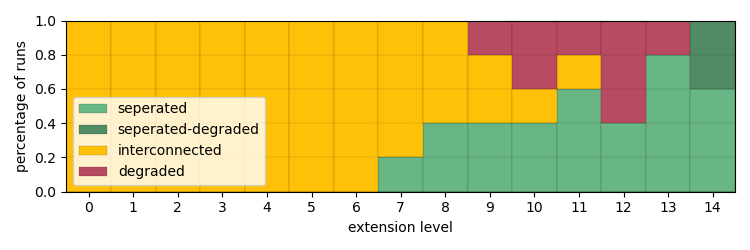
\includegraphics[width=1.0\linewidth]{3-layer-histogram-split-behaviour.png}
\caption[Separation/Degradation Stacked Area Chart (3 hidden layers)]{
A proportional stacked area chart showing the ratio of training runs in each category.
The x-axis shows the extension level, and the y-axis shows the relative amount of networks in each category, stacked. (3 hidden layers)
}\label{fig:3layer-histogram}
\end{figure}
In figure~\ref{fig:3layer-histogram} the same graph for the three-layer network is shown.
A similar effect occurs but unlike the single-layer network, the network does not stop to separate in the range that was tested. 

%%%%%%%%%%%%%%%%%%%%%%%%%%%%%%%%%%%%%%%

\subsection{When Do Networks Separate?}
Do the networks always start to separate at the same pruning level or with the same number of unpruned parameters?
This question is investigated in the following paragraph.
Interestingly, when extending the network to higher levels, it tends to separate into earlier pruning levels.
This results in an increased number of available weights to the network at the iteration they separated.
\begin{figure}[t] % Active/Available d=2
    \centering
    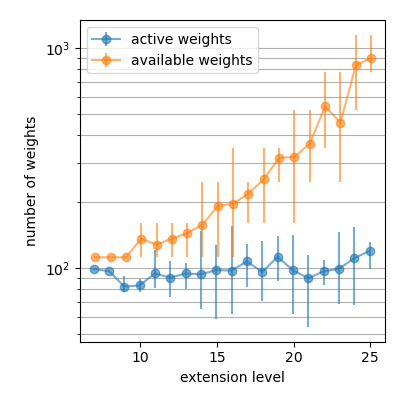
\includegraphics[width=.6\linewidth]{2-layer-active-available-at-split-log.png}
    \caption[Comparing active and available weights (2 hidden layers)]{
    The number of active weights (blue) and the number of available weights (orange).
    Each dot is an average of four training runs.
    The error bars indicate the minimum and maximum of the runs.
    Log scale. (2 hidden layers)
    }\label{fig:2l-active-split}
\end{figure}
Figure~\ref{fig:2l-active-split} depicts the number of available/unpruned weights in orange and the number of active weights in blue, for the different extension levels of networks with two hidden layers.
Each dot represents the average number of active or available weights at the exact iteration where the network is separated.
Only training runs where the network separates are taken into account.
For each extension level, the training run was repeated with four different seeds for the initialization of the network weights.
On the x-axis, the extension level of the network is displayed, which is also the number of pruning levels the network goes through.
The more extension levels, the larger the network.
The error bars indicate the maximum and minimum values of the different runs.
The graph is shown on a logarithmic scale.

A visible trend is the exponential increase of the number of available weights at the level where the network separates (orange).
This comes from the fact that the networks separate in earlier iterations, where there are more available weights.
Interestingly, the number of active weights does not experience comparable growth when the network is extended more.
Active weights are the weights that are contained in the active subgraph $\mathcal{G}_a$, that was introduced in chapter~\ref{chapter:method}.
It increases slightly but almost remains flat, covering a narrow range of around $80$ to $120$ weights, while the available weights grow from $120$ to around $900$.
This data indicates that the number of active weights might be an important quantity to network separation.
Since the active subgraph $\mathcal{G}_a$ is indeed the graph that is used to evaluate network separation, this seems plausible.
 
% 1 hidden layer
\begin{figure}[t] % Active/Available d=1
    \centering
    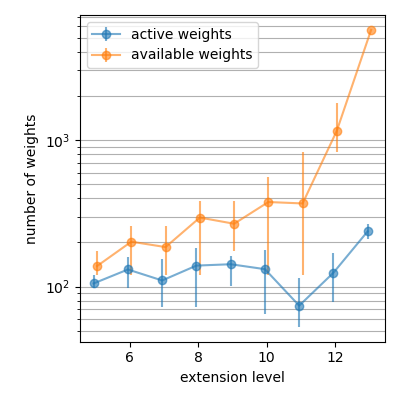
\includegraphics[width=0.6\linewidth]{1-layer-active-available-at-split-log.png}
    \caption[Comparing active and available weights (1 hidden layer)]{
    The number of active weights (blue) and the number of available weights (orange).
    Each dot is an average of four training runs.
    The error bars indicate the minimum and maximum of the runs.
    Log scale.  (1 hidden layer)
}\label{fig:1layer-active}
\end{figure}

When looking at the graph of the architectures with one hidden layer, this effect is even more dramatic, which is shown in figure~\ref{fig:1layer-active}.
Similarly to the experiment with two layers, the networks separate in earlier iterations when they are larger and have more pruning levels.
The number of active weights remains in a fairly tight range between $70$ and $120$ active weights, while the number of available weights goes from around $125$ to over $1400$.
Notably, as shown in figure~\ref{fig:1layer-histogram}, the network does not separate anymore after the 13th extension level.
At the 13th level, only around $10$ percent of the weights in the network are active at the separation iteration.

\begin{figure}[t] % Active/Available d=1
    \centering
    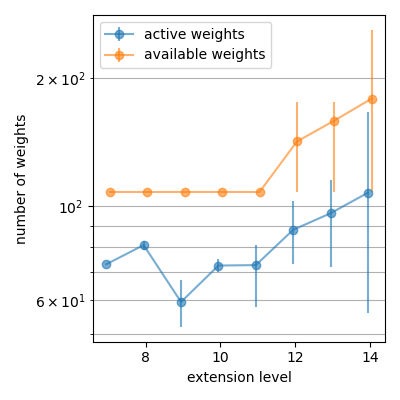
\includegraphics[width=0.5\linewidth]{3-layer-active-available-at-split-log.png}
    \caption[Comparing active and available weights (3 hidden layers)]{
    The number of active weights (blue) and the number of available weights (orange).
    Each dot is an average of four training runs.
    The error bars indicate the minimum and maximum of the runs.
    Log scale.  (3 hidden layers)
    }\label{fig:3layer-active}
\end{figure}

When considering the network with three hidden layers, a similar effect is visible, however significantly less pronounced.
Figure~\ref{fig:3layer-active} depicts the number of active weights and the number of available weights of the three-layer architectures with different extension levels.
The networks at extension level 7 until 11 all split at the last pruning level, which can be deducted by the number of available parameters which is equal to the pruning target of 108.
The number of active weights is slightly lower than in the other experiments.
The data indicates that separating a three-layer network with the same number of available parameters is less likely than a two or a one-layer network because the number of available weights does not grow as quickly.
Also when looking at the number of active weights at the level where the three-layer networks separate, the numbers are significantly lower compared to the other architectures.

\subsection{What Makes Networks Separate?}
As seen in figure~\ref{fig:2laxer-histogram}, the networks with two hidden layers start to split at 7 extension levels and a network shape of $(4,38,38,2)$, with 1672 weights.
However, it is not obvious what the main contributor to network separation is.
To gain a better understanding of that phenomenon an experiment was conducted that compares different combinations of pruning levels, network size, and pruning rate for the two-layer architectures.
For this experiment, four architectures were selected.
One network with shape $(4,31,31,2)$ (extension level 6), which did not separate in any run.
Networks with $38$ and $48$ hidden neurons (extension levels 7 and 8), where only one in four networks separated.
And finally a network with 57 hidden neurons, where all four runs have separated.
This range of architectures is assumed to encompass a critical area, due to the change in separation behavior.
Further, each of the four architectures was trained with $0$ to $10$ pruning levels.
The pruning target is fixed at $112$, such that all networks end up at the same number of unpruned parameters after the last pruning level.
Therefore, the pruning rate is variable depending on network size and number of levels.
The larger the network, the higher the pruning rate, given a fixed number of iterations.
Each training run with a combination of network size and number of pruning levels was repeated four times, with different seeds for the network initialization.

\begin{figure}[ht] % what influences separation : size
    \centering
    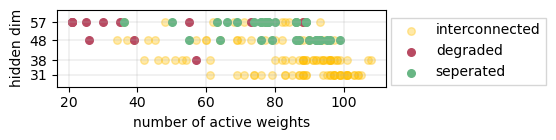
\includegraphics[width=1.0\linewidth]{grid-2-layer-eval-abs.png}
    \caption[Influence of network size on separation]{
        The influence of network size on separation is shown.
        Each dot is a single training run, color-coded by category.
        }\label{fig:grid-1}
\end{figure}

In figure~\ref{fig:grid-1} the impact of network size is demonstrated.
On the y-axis, the size of the network is encoded by its hidden dimension.
On the x-axis, the number of active weights after the last pruning level is depicted.
Each dot represents one training run.
The colors denote if the network separated, degraded or remained interconnected.
Regarding the two smaller networks with hidden dimensions $31$ and $38$, none of the networks separated. 
Increasing the number of pruning levels and decreasing the pruning rate did not result in separated networks.
On the other hand, the two larger networks separate numerous times.
These results indicate, that there is a phase change in the ability of the network to separate.
A certain level of overparameterization seems to be necessary for the network to separate well.

\begin{figure}[ht] % what influences separation : plevels
    \centering
    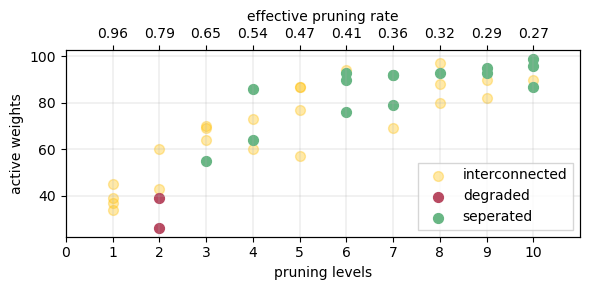
\includegraphics[width=1.0\linewidth]{grid-2-layer-pruning-rate-48-hd.png}
    \caption[Influence of pruning rate on separation]{
        Influence of the pruning rate on separation is shown.
        Each dot is a single training run, color-coded by category.
    }\label{fig:grid-2}
\end{figure}

To investigate the influence of pruning levels and pruning rate, the separation behavior of the network with hidden dimension 48 is depicted in figure~\ref{fig:grid-2}.
Since the pruning target and the network size are fixed, the pruning rate has to change when increasing the number of pruning levels.
On the bottom x-axis, the number of pruning levels is depicted, and on the top x-axis, is the corresponding pruning rate.
On the y-axis, the number of active weights after all pruning levels is depicted.
With more pruning levels and a lower pruning rate, the network is more likely to separate.
Also, a seemingly contradicting trend to figure~\ref{fig:collateral_damage} is visible, namely that the number of active weights increases with more pruning levels.
The difference to the previous experiment is, that while the number of pruning levels increases in both cases, the pruning rate decreases with more pruning levels in this experiment, which is visible in figure~\ref{fig:grid-2}. In the experiment depicted in figure~\ref{fig:collateral_damage}, the pruning rate is constant, while the network size increases.

However, this data also indicates that there is a certain phase change in the likelihood of the network separating.
Since the pruning rate and the number of pruning levels are two tightly interlinked parameters, it is hard to examine them in isolation.
The largest pruning rate where a network separated was $\sim0.65$. 
With pruning rates lower than $\sim0.41$, the networks consistently separate.
The data indicates that more pruning levels with lower pruning rates are generally favorable to network separation.
\textcite{LTH} already note that iterative pruning leads to smaller lottery tickets than one-shot pruning.
It is reasonable to assume, that the same phenomenon takes place concerning network separation.
Less pruning levels versus lower pruning rates represent a trade-off between favorable conditions and computational cost.

\subsection{How Do Networks Separate?}
Another open question is, what the process of separation looks like.
In the beginning, when the network is fully connected, it is not yet clear which weight and neuron belongs to which task.
One available option, however, is to view the network from the perspectives of the inputs and outputs.
The input and output features are the only parts of the network that can already be associated with a task when it is fully connected.
This enables determining the degree to which the neighboring layers have separated as well.

For instance, regarding the simple Moons-Circles dataset, there are two output neurons.
Each neuron in the penultimate layer has two outgoing connections: one to the Circles-output and one to the Moons-output.
When one of the connections is pruned, the neuron and all its incoming connections are automatically part of the task the unpruned weight is connected to.
The number of neurons in any given layer that are only connected to one of the outputs of one task is denoted $N_{decided}$.
The number of neurons that are connected to both tasks is denoted $N_{undecided}$.
The degree of separation is determined by 
\[ \frac{N_{decided}}{N_{decided}+N_{undecided}} \]
This calculation can be done from either the side of the inputs or the outputs and it works in the same way.
Only if a layer has at least one neuron that has \textit{decided} to which task it belongs, neurons in the next layer can \textit{decide} as well.

\begin{figure}[t] % Layer separation from outputs
    \centering
    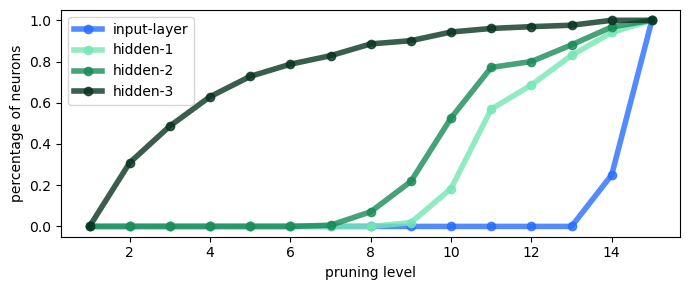
\includegraphics[width=0.9\linewidth]{output-view.png}
    \caption[Separation from the view of output neurons]{
    The degree to which neurons in hidden layers can be attributed to a task over the pruning levels; calculated by the connectivity to the output neurons.
    Each line shows the percentage of weights attributable to a task.
    The x-axis shows the pruning levels from 0, where the network is fully connected to 15, where the network separated.
    }\label{fig:outview}
\end{figure}

\begin{figure}[t] % Layer separation from inputs
    \centering
    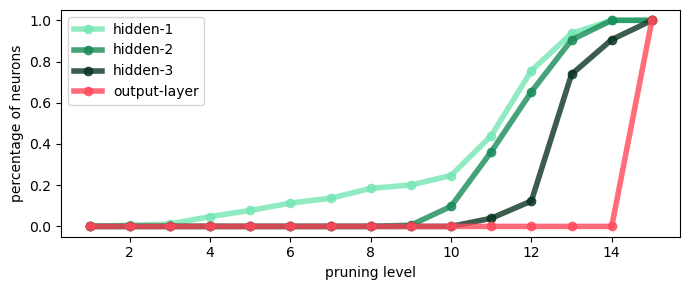
\includegraphics[width=0.9\linewidth]{input-view.png}
    \caption[Separation from the view of input neurons]{
        The degree to which neurons in hidden layers can be attributed to a task over the pruning levels; calculated by the connectivity to the input features.
        Each line shows the percentage of weights attributable to a task.
        The x-axis shows the pruning levels from 0, where the network is fully connected to 15, where the network separated.
    }\label{fig:inview}
\end{figure}

In figure~\ref{fig:outview} the degree of separation is displayed for each layer from the view of the outputs.
On the x-axis, the pruning levels are displayed and on the y-axis the percentage of neurons that can be attributed to a task.
The network in this case was taken from the experiment with three hidden layers.
It separates at iteration 15.
In the first iteration, none of the layers were separated.
Already by the second iteration, around $30$\% of the neurons in the last hidden layer (hidden-3) belong to only one task.
This increase in the degree of separation of this layer resembles a logarithmic growth.
At iteration 7, where already $\sim80$\% of neurons in the last hidden layer belong to a task, the penultimate hidden layer (hidden-2) starts to separate.
With one iteration delay, the next hidden layer (hidden-1) starts to separate.
It tracks the layer \textit{hidden-2} in its rapid, s-curve-shaped growth.
Only at iteration 14, when over $90$\% of neurons are already attributable to a task, the input layer separates.
In this case, the separation describes the perspective from the outputs.
It does not take into account the knowledge, of which input neuron belongs to which task.

The same network but from the view of the inputs is displayed in figure~\ref{fig:inview}.
On the x-axis, the pruning levels are displayed and on the y-axis the percentage of neurons that can be attributed to a task.
In this case, the separation is significantly slower in the beginning.
After iteration 10, the separation speeds up at iteration 15, the network is completely separated.
The difference in the degree of separation, depending on the point of view, could have several reasons.
It could be that the slower separation is due to the fact, that there are four inputs and only two outputs.
Therefore, for the neurons to be only connected to the inputs of one task, two instead of one weights have to be pruned.
Another possibility is that the weights in the first layer are higher in magnitude than the weights in the last layer.
This would result in stronger pruning in the last layer.

\subsection{Performance of Separated Networks}
One remaining question is if the networks still perform well when they separate.
Are they better, equal, or worse in terms of the validation loss, compared to the other networks?

\begin{figure}[t]
    \centering
    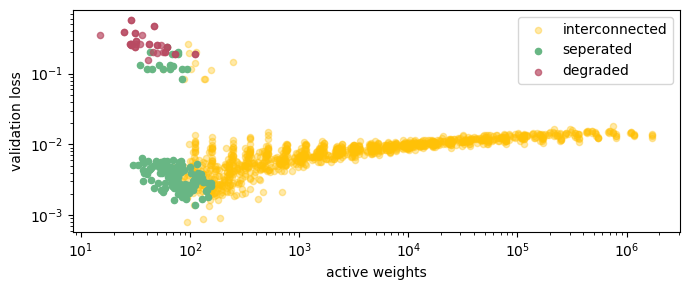
\includegraphics[width=0.9\linewidth]{performance.png}
    \caption[Performance of winning tickets]{
        The performance of winning tickets, color-coded by category.
        Winning tickets that separated are shown in green.
        Log scale. (2 hidden layers)
    }\label{fig:performance}
\end{figure}

To investigate the performance, the validation loss from the experiment with two hidden layers described in paragraph~\ref{two-hidden} was used.
In figure~\ref{fig:performance}, the validation loss is depicted on the y-axis.
On the x-axis, the number of active weights is displayed.
On the y-axis, the validation loss is shown.
Each dot represents a network at one stage.
An experiment with 20 pruning levels is shown with 20 dots in this figure.
The color refers to the state of the network at the iteration.
The color of the point represents if the network was interconnected (yellow), separated (green), or degraded (red) at the iteration the point refers to.
The loss value is calculated after the training and before the pruning of each iteration, as shown in the code snippet~\ref{code:imp}.

The bending line of yellow points demonstrates the consistent performance of the networks during the early iterations.
Likely due to early stopping, the networks remain at a validation loss of around $0.01$.
The loss decreases slightly over the pruning iterations.
A visible cluster of green dots sits at the end of the yellow line.
These dots represent the networks that are separated.
The iterations where the networks are separated are amongst the networks with the lowest loss.
This indicates that the separation of the networks is not merely a consequence of pruning to extremely high sparsities.
Rather, the separated networks still represent a well-performing function, even amongst the best-performing networks overall.

Interestingly, there is a second distinct cluster of networks.
It sits at the same number of active weights, however with significantly higher loss.
This cluster contains interconnected, separated, and degraded networks at seemingly even ratios.
Since the experiments were stopped as soon as a network degraded, the red points refer to losses immediately after the network degraded.
Even though the cluster looks compact along the y-axis it covers a fairly large range between 0.08 and 0.56 loss. These losses correspond to an accuracy of roughly $95$\% and $65$\% respectively.
The separated and interconnected networks still generally inhabit an area with lower loss than the degraded networks.

\subsection{Inactive Parameters and Zombies}
As introduced in chapter~\ref{chapter:method}, there are four different kinds of states the parameters of the network can be in.
Parameters can be pruned, inactive, active or zombies.
The number of pruned parameters increases at a predictable rate over the training run.
How do the other kinds of parameters evolve?
With the two-layer architectures extended over several levels as shown in table~\ref{tab:trajectory}, the inactive and zombie parameters are investigated.

\begin{figure}[t]
    \centering
    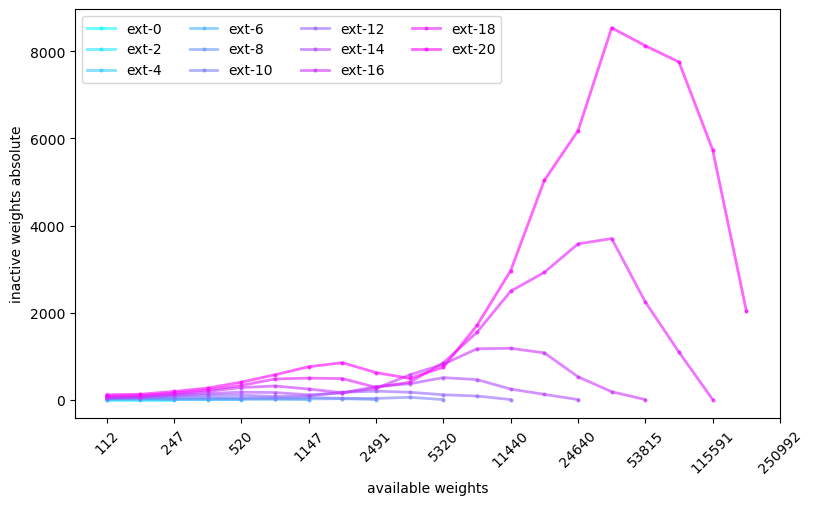
\includegraphics[width=.9\linewidth]{inactive-abs-2l.png}
    \caption[Inactive Weights during training runs, absolute]{
        The number of inactive weights over the training runs. 
        Each line represents a different extension level. 
        The x-axis shows the available weights and the y-axis shows the absolute number of inactive weights.
    }\label{fig:inactive-abs}
\end{figure}

In figure~\ref{fig:inactive-abs}, the absolute number of inactive weights is displayed.
Every line represents a certain network size, indicated by the extension level (ext-$i$).
Further, the lines are averages of four training runs with different seeds for model initialization.
On the x-axis, the number of available parameters of the network is displayed.
On the y-axis, the number of inactive weights in the network is shown.
Networks that were extended to higher levels, experienced more pruning levels and therefore have longer lines in the graph.
It is visible, that the number of inactive weights is larger with larger networks.
Especially at the earlier pruning iterations of each network, the numbers grow and subsequently fall significantly.
However, due to the reduction in the overall network size, this is to be expected.

\begin{figure}[t]
    \centering
    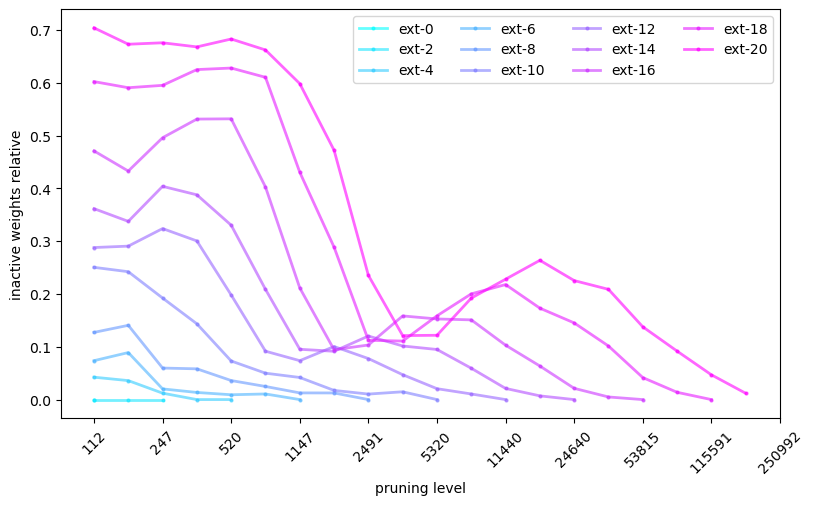
\includegraphics[width=.9\linewidth]{inactive-rel-2l.png}
    \caption[Inactive Weights during training runs, relative]{
        The number of inactive weights over the training runs. 
        Each line represents a different extension level. 
        The x-axis shows the available weights and the y-axis shows the relative number of inactive weights.
        }\label{fig:inactive-rel}
\end{figure}
The same graph, however with the relative amount of inactive weights is shown in figure~\ref{fig:inactive-rel}.
Here, a different trend is visible.
As the number of weights in the network decreases, the percentage of inactive weights generally increases.
Interestingly, this increase is not steady.
With larger network sizes, a distinct pattern emerges.
The ratio of inactive weights increases to a certain level and subsequently decreases, which results in a visible bump in the line.
Afterward, the value increases again until it flattens off.
The larger the network, the larger the number of inactive weights at the final pruning levels.
With smaller networks, this pattern cannot be seen.

\begin{figure}
    \centering
    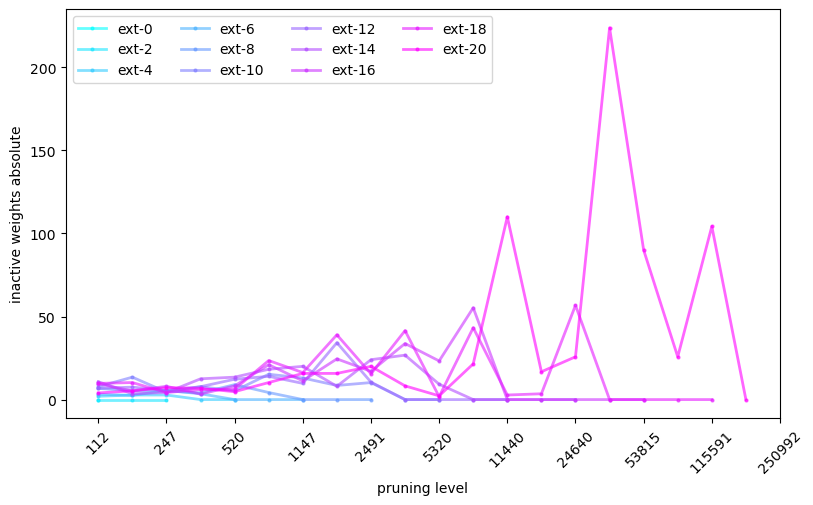
\includegraphics[width=.9\linewidth]{zombie-abs-2l.png}
    \caption[Zombie weights during training runs, absolute]{
    The number of zombie weights over the training runs. 
    Each line represents a different extension level. 
    The x-axis shows the available weights and the y-axis shows the absolute number of zombie weights.
    }\label{fig:zombie-abs}
\end{figure}

When examining the number of zombie weights in the network, a different pattern is visible.
In figure~\ref{fig:zombie-abs}, the absolute number of zombie weights is displayed for the same networks.
Similarly to figure~\ref{fig:inactive-abs}, the number of zombies is larger when the networks have more parameters available.
However, the number of zombie weights is significantly less than the number of inactive weights.

\begin{figure}
    \centering
    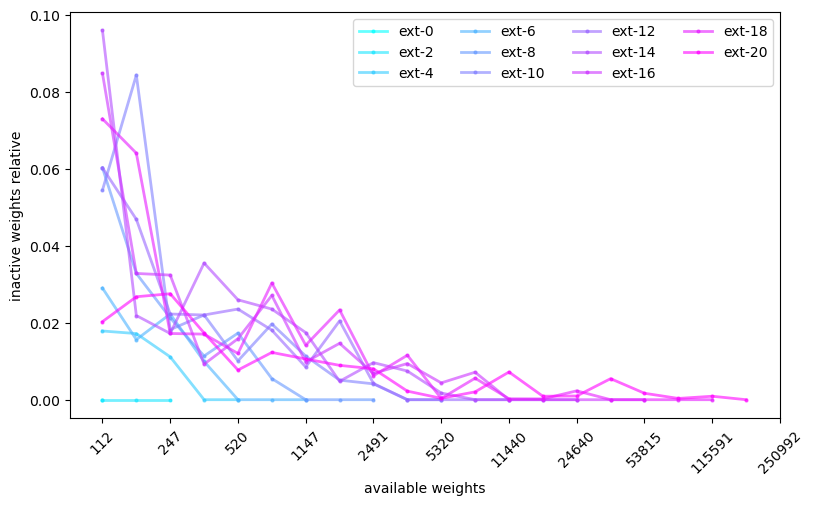
\includegraphics[width=.9\linewidth]{zombie-rel-2l.png}
    \caption[Zombie weights during training runs, relative]{
        The number of zombie weights over the training runs. 
        Each line represents a different extension level. 
        The x-axis shows the available weights and the y-axis shows the relative number of zombie weights.
    }\label{fig:zombie-rel}
\end{figure}

Again, a more interesting view is the relative amount.
Figure~\ref{fig:zombie-rel} shows the relative amount of zombie weights, compared to all other unpruned weights.
It generally increases, the more the network is pruned.
Interestingly, the values do not seem to tail off as the ratio of inactive weights in figure~\ref{fig:inactive-rel}.
When comparing zombie weights and inactive weights, it is clear that inactive weights represent a significantly larger fraction of all weights of the network.
Why this is the case is an interesting question for future research in this direction.

\section{Experiments on the MNIST-Fashion-MNIST Dataset}
Due to the success of IMP in separating the neural network on the Moons-Circles dataset, the same was attempted on the more realistic MNIST-Fashion-MNIST dataset described in paragraph~\ref{sec:mnist}.
The experiments cannot be executed as systematically as before, due to significantly higher computational cost.
However, with experience gained from previous experiments, it was indeed possible to find separated networks.
The hyperparameters are mostly the same as in the previous experiments.
The network is trained with the ADAM optimizer and a learning rate of $0.001$.
Additionally, a larger batch size of 512 is selected, since the data is more diverse and there are significantly more samples.

The dataset includes 1568 input features and 20 output features.
A network with shape $(1568, 784, 392, 20)$ was used for these experiments.
The architecture was selected to resemble the LeNet architecture used in \autocite{LTH} on the MNIST dataset.
The LeNet architecture has a shape of $(784, 300, 100, 10)$.
In preliminary experiments, the networks separated at significantly larger numbers of parameters than in the Moons-Circles experiments.
Therefore, the pruning target was set to 600.
For the training runs, 20 pruning levels were selected, which resulted in a pruning rate of $p=0.3247$, similar to the experiments on the Moons-Circles dataset.
For the first experiments, the data was normalized like the Moons-Circles dataset, namely to zero mean and unit variance along each pixel.

\subsubsection{Adapting Loss Function}
To enable training with this dataset, the loss has to be adapted.
For classification with more than two classes, the categorical cross entropy can be used.
For each of the tasks in the concatenated dataset, the loss is computed separately.
The total loss is simply the sum of the losses from each task.

Concretely, let $\mathbf{\hat y_{mnist}} = \left[\hat y_1, \dots, \hat y_{10}\right]$ be the output logits of the network that relates to the MNIST dataset and $\mathbf{\hat y_{fashion}} = \left[\hat y_{11}, \dots, \hat y_{20}\right]$ to the Fashion-MNIST dataset.
Together, they form the network output $\mathbf{\hat y} = \left[\hat y_1, \dots, \hat y_{20}\right]$
The true labels $\mathbf{y}$ similarly contain $\mathbf{y_{mnist}}$ and$\mathbf{y_{fashion}}$ respectively.
Let $\mathcal{L} (\mathbf{\hat y}, \mathbf{y})$ be the loss of the network output $\mathbf{\hat y}$ and the true labels $\mathbf{y}$.
The total loss $\mathcal{L}$ of the network is calculated as follows:
\[
\mathcal{L}  (\mathbf{\hat y}, \mathbf{y})
= \ell  (\mathbf{\hat y_{mnist}}, \mathbf{y_{mnist}})
+ \ell (\mathbf{\hat y_{fashion}}, \mathbf{y_{fashion}})
\]
, where $\ell$ represents the categorical cross-entropy loss.

\subsubsection{Adapting Network Degradation}
In paragraph~\ref{sec:taskmatch} network separation and network degradation were introduced.
When trained on the Moons-Circles dataset from paragraph~\ref{sec:independece_dataset}, a network counts as degraded when any of the inputs or outputs are cut off from the network, since all inputs and outputs are relevant for the success of the network.
However, regarding the MNIST-Fashion-MNIST dataset, this is not the case.
Many of the input features do not carry information, for example, the outer frame of the MNIST images.
Therefore, it is to be expected that all connections to these inputs may be pruned.
This would likely lead to unwanted network degradation.

The network only counts as degraded, if an output feature is completely cut off.
In this case, the network cannot function properly anymore, since one class cannot be predicted any longer.
Consequently, the output-coverage is used as a basis to evaluate degradation.

\subsection{Results}
With the described setup, the network was trained with three different seeds for the weight initialization.
Figure~\ref{fig:mnist-acc} shows the accuracy of three runs with the same hyperparameters but different seeds on the MNIST-Fashion-MNIST dataset.
On the x-axis, the number of active weights is displayed.
On the y-axis, the accuracy is shown.
Each line represents one run.
The red star indicates where the networks separated.
The iteration where the networks separate is also always the last because after separation occurs, the training is stopped.
When the networks separate, the accuracy already is significantly lower than at the peak.
The best accuracy of a separated network amongst the shown runs is $\sim86$ percent.

\begin{figure}
    \centering
    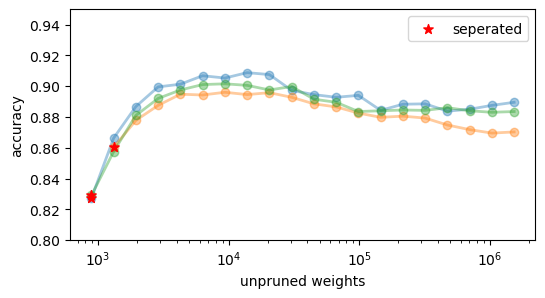
\includegraphics[width=.7\linewidth]{mnist-acc-largest-784-392.png}
    \caption[Performance and Separation on MNIST-Fashion-MNIST]{The performance of three training runs with different seeds. 
    Each line represents one training run, where the hyperparameters are the same.
    The performance where the network separates is indicated by the red star.
    The x-axis shows the number of available/unpruned weights on a logarithmic scale.
    The y-axis shows the accuracy.
    }\label{fig:mnist-acc}
\end{figure}

\begin{figure}
    \centering
    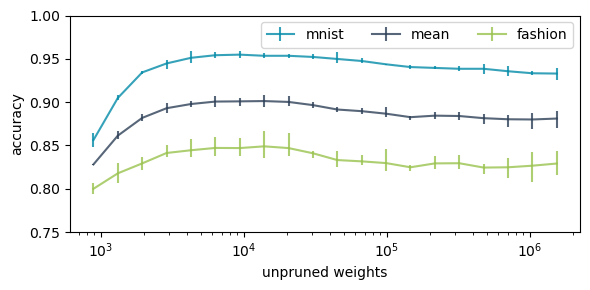
\includegraphics[width=.7\linewidth]{taskwise-acc.png}
    \caption[Taskwise performance]{
        The performance of the separate tasks in the network.
        Each line shows the average, minimum and maximum accuracy of the three repeated training runs.
        The lines show the accuracy of the MNIST task (blue), the Fashion-MNIST task (green) and the average of both (dark blue).
    }\label{fig:taskwise-acc}
\end{figure}

The data shown in figure~\ref{fig:mnist-acc} represents the average accuracy of both tasks.
The data in figure~\ref{fig:taskwise-acc} shows the accuracy of the tasks separately.
Each line is an average of the three runs with different seeds.
The error bars indicate minimum and maximum values.
On the x-axis, the number of active weights is displayed.
On the y-axis, the accuracy is shown.

Since the tasks are not the same, it is to be expected that they do not exhibit the same performance.
The accuracy achieved on the MNIST task is more than $10$~percent higher than on the Fashion MNIST task.
Interestingly, when the number of parameters gets lower, the performance on the MNIST task worsens significantly faster than for the Fashion MNIST task.
The performance of the network is not competitive anymore at the time it separates.
However, the experiments shown here are only preliminary.
The networks indeed separate consistently, and they do far beyond trivial accuracies.
This gives reason to believe, that the separation can be achieved at competitive accuracy with improved hyperparameters or slight adaptations to the training.
This, however, is not pursued in the scope of this thesis.
The separation by itself, at non-trivial accuracy is considered a useful insight into the structure of the network.

\subsection{Connectivity of the input layer}
An interesting finding of \textcite{LTH} was, that certain neurons in the input layer retain significantly more incoming connections than others.
They find this to be the case with winning tickets trained on MNIST and attribute this to the fact that certain pixels of the MNIST dataset do not contain any useful information.
In figure~\ref{fig:mnist-input-variance} the pixel-wise mean and variance of the MNIST dataset is shown.
Since the digits are centered in the image, there is a frame where there is little to no variance and where the values are on average close to zero.

\begin{figure}[!ht] % mnist variance
    \centering 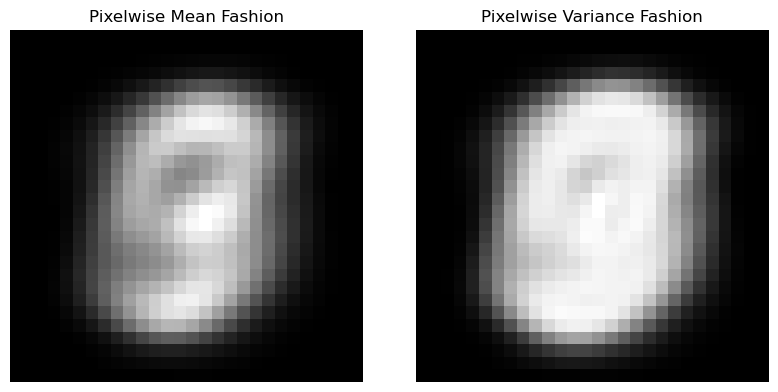
\includegraphics[width=.7\linewidth]{mnist_mean_variance.png}
    \caption[Mean and Variance MNIST]{
    The mean (left) and variance (right) of each pixel in the MNIST dataset
    }\label{fig:mnist-input-variance}
\end{figure}
\begin{figure}[!ht] % fashion variance
    \centering 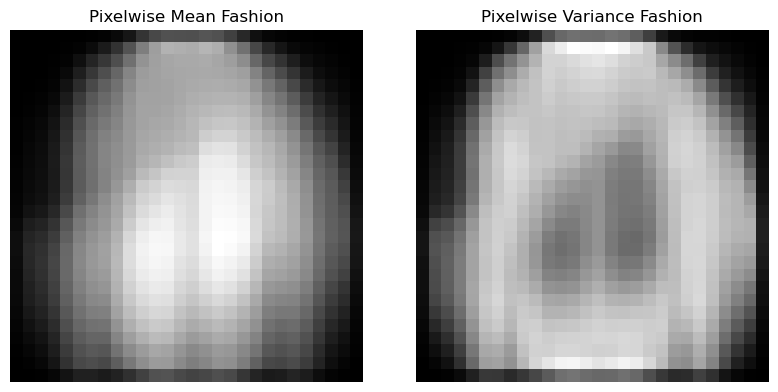
\includegraphics[width=.7\linewidth]{fashion_mnist_mean_variance.png}
    \caption[Mean and Variance Fashion-MNIST]{
        The mean (left) and variance (right) of each pixel in the Fashion-MNIST dataset
        }\label{fig:fashion-input-variance}
\end{figure}

A similar effect is visible with the Fashion MNIST dataset as seen in figure~\ref{fig:fashion-input-variance}.
For the Fashion-MNIST dataset, the frame is notably smaller and there are pixels with significant mean and variance that lie on the outermost pixel row of the image.
For each of the datasets, a neural network with the same architecture as in \autocite{LTH} was used, namely the LeNet architecture with a shape of $(784,300,100,10)$.
The networks were pruned for 18 pruning levels to a pruning target of {$600$}.

Figure~\ref{fig:mnist-heatmap} shows the connectivity to the input layer at different pruning iterations.
The shape of the digits as seen in figure~\ref{fig:mnist-input-variance} is distinctly visible over many pruning levels.
This means that there tend to be more outgoing connections of pixels that are in the high-variance or high-mean area of the image.
At pruning level 11 where only 2 percent of all weights are active, many pixels on the outer frame of the image do not have any connection left.
At iteration 15, most of the pixels on the outer frame have been completely disconnected.
However, there remain some pixels on the outer frame that hold onto the connections, even though they do not carry any information.
This suggests that there is an increased likelihood of disconnecting from pixels with no information.
Due to the probabilistic nature of training and network initialization, there may remain connections to zero-information inputs.

\begin{figure}[!htb] % MNIST attention heatmap
    \centering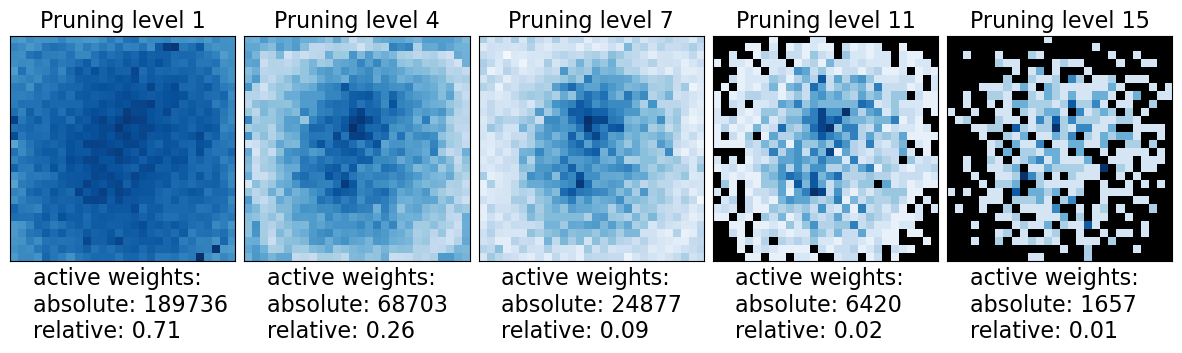
\includegraphics[width=1.\linewidth]{mnist_input_attention_active.png}
    \caption[Pixel connectivity MNIST]{
        Heatmap of the number of outgoing connections of each input pixel of the MNIST dataset, over several pruning levels.
        }\label{fig:mnist-heatmap}
\end{figure}
\begin{figure}[!htb] % Fashion attention heatmap
    \centering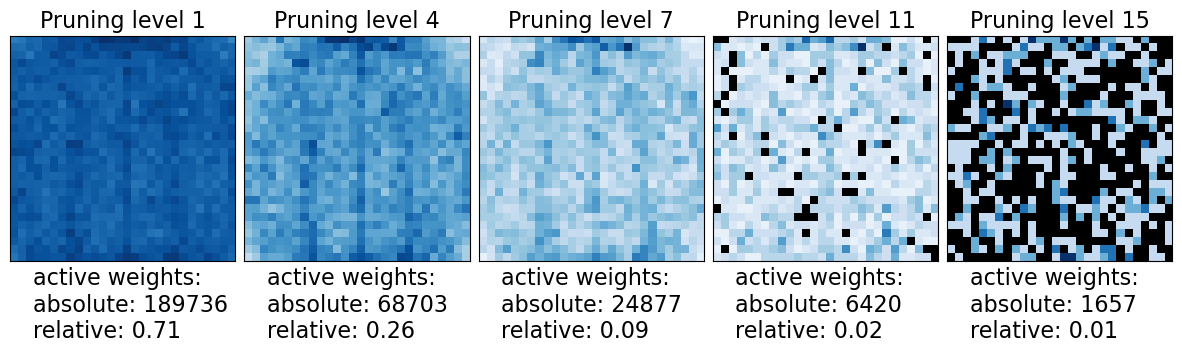
\includegraphics[width=1.\linewidth]{fashion_input_attention_active.png}
    \caption[Pixel connectivity Fashion-MNIST]{
        Heatmap of the number of outgoing connections of each input pixel of the Fashion-MNIST dataset, over several pruning levels.
        }\label{fig:fashion-heatmap}
\end{figure}

Figure~\ref{fig:fashion-heatmap} shows this for the Fashion dataset.
In early iterations, a pattern can be detected that resembles the overall shape of some fashion items.
Further, a line in the center with more connections is visible.
This might be the case because many items have characteristic lines in the center, like trousers, shirts or jackets.
The line is also visible in the mean and variance of the dataset as shown in figure~\ref{fig:fashion-input-variance}.
At pruning levels one, four and seven, the number of connections per pixel shows a similar shape to the mean and variance of the dataset.
At iterations four and seven, there is a horizontal bar of strongly connected pixels in the center of the upper edge of the image. 
This bar is also visible in the pixel-wise variance of the dataset, which indicates a connection between variance and connectivity.
However, with the Fashion dataset, the pattern disappears in later iterations.
At pruning level 11, there is no pattern visible anymore and at iteration 15, many of the center pixels are completely disconnected.

One possible explanation for the clearer pattern in the MNIST dataset is that the different classes are more similar and take up a more compact area in the image, as seen in figure~\ref{fig:mnist-input-variance}.
Also, the performance on the MNIST dataset is better than on the Fashion dataset, with the same hyperparameters.
This might indicate, that the Fashion dataset is harder to learn for the {MLP}, which could also impact the connectivity of the input layer.

%%% old
\begin{figure}[ht] % mnist-fashion-mnist connectivity
    \centering
    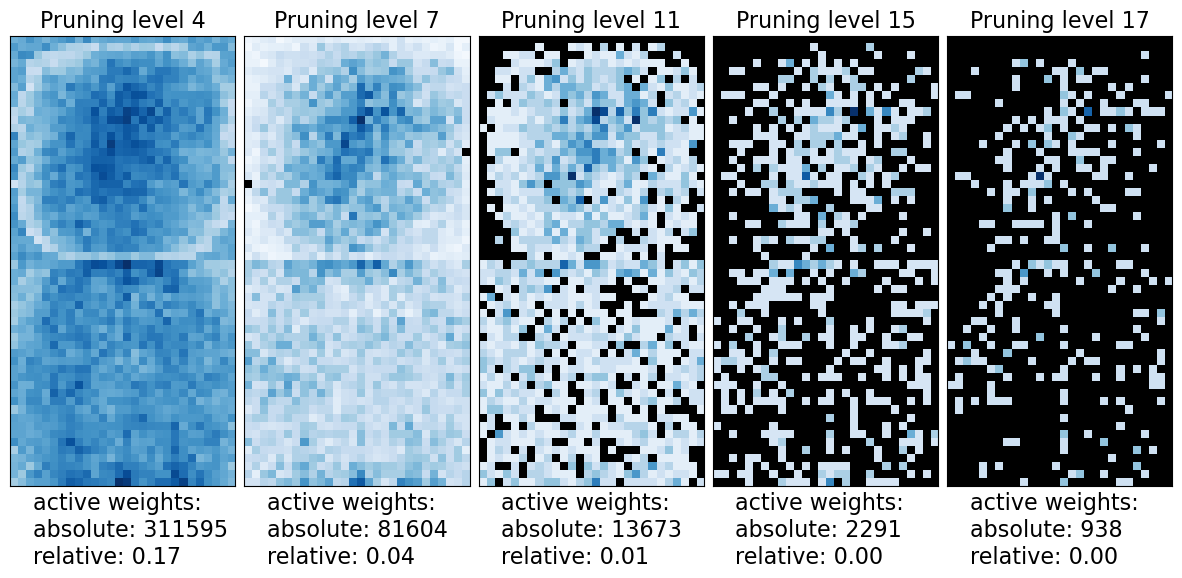
\includegraphics[width=1.\linewidth]{mnist_fashion_mnist_input_attention_active.png}
    \caption[Pixel connectivity MNIST-Fashion-MNIST]{
    Heatmap of the number of outgoing connections of each input pixel of the MNIST-Fashion-MNIST dataset, over several pruning levels.}\label{fig:mnist-fashion-map}
\end{figure}

When examining a training run on the MNIST-Fashion-MNIST set with a network of shape $(1568, 784, 392, 20)$, the same patterns emerge.
In figure~\ref{fig:mnist-fashion-map}, the connectivity on the concatenated dataset is shown.
The images are shown as stacked, where the MNIST image is on top and the Fashion image is on the bottom.
On the MNIST image, the same pattern as before is visible.
In the Fashion image, parts of the pattern are visible but less pronounced.
Given that both tasks are trained at the same time, it might be that the hyperparameters are better suited for MNIST than for Fashion-{MNIST}.
After iteration 17, which is the rightmost image, the network separated.
The connectivity is severely degraded at this point even though the network has an accuracy of $83$ percent at that iteration.
This further advances the point, that the network in this example separated very late in the process.
Improved hyperparameters and training techniques could lead to separation at earlier iterations.
\chapter{Conclusion}\label{chapter:conclusion} 

In this thesis, the structure of winning tickets created with iterative magnitude pruning was analyzed empirically.
It was shown, that feed-forward neural networks consistently separated into two independent subnetworks by iterative magnitude pruning when trained on a dataset with independent tasks.
With the right conditions, such as a large enough network and enough pruning levels, the networks consistently separate over different pruning rates and network sizes.
The separation was tested on custom datasets with two independent tasks.
Systematic experiments were conducted on the Moons-Circles dataset, a toy dataset that contains two independent tasks.
Due to the success of the method on the toy task, experiments were also conducted on the MNIST-Fashion-MNIST dataset, which is significantly more realistic.
In both cases, neural networks were found to separate with non-trivial accuracy and without any regularization techniques.

These results indicate that iterative magnitude pruning (IMP) indeed produces winning tickets with meaningful structure.
Also, the results indicate that there is a probabilistic element to the degree to which these structures come to light.

\section{Limitations}
The findings of this thesis are empirical, and due the the scope and scale of the thesis, there are numerous untested scenarios.
The experiments were only conducted on toy datasets and on MNIST-Fashion-MNIST which might also be counted as a toy dataset.
Whether the findings remain true for larger and more realistic tasks remains an open question.

Another limitation is the restriction to datasets with similarly complex tasks.
Scenarios with tasks that vary in size or complexity were not tested in this thesis.
Further, only fully connected networks were tested.
Other architectures such as convolutional neural networks were not used in any experiments.
All of the limitations invite for future work on this topic.

\section{Discussion}
The experiments in this thesis demonstrate that iterative magnitude pruning finds independent subnetworks.
This can be valuable for understanding what the structure of winning tickets represents.
Further, it could also be valuable for machine learning interpretability.
A winning ticket could be trained and if independent networks occur, it could hint at independence in the dataset.
The same might be true for other types of semantic structure, like feature sharing or compositionality.

\section{Future Work}
An interesting avenue for future research in this line of work would be to examine the numerous other variants for finding sparse subnetworks, like Rare Gems~\autocite{RareGems}.
Would they also separate? And if so, would they separate earlier or with better performance still?
Many methods that enhance iterative magnitude pruning like learning rate schedules and resetting to later training iterations, as well as L1 and L2-regularization could also be tested.
Similar to the work by \textcite{BIMT}, other semantic structures of the data might be considered, like compositionality or weight sharing.
One could examine the methods on larger and more realistic datasets like CIFAR-10 or ImageNet.
Finally, the findings from this thesis could be translated into convolutional neural net architectures, where network separation has not been tested yet.
\printbibliography[
    title={Bibliography},
    heading=bibintoc
]

% additional stuff
\pagenumbering{roman}
\newpage

\listoffigures
\addcontentsline{toc}{chapter}{List of Figures}
\newpage

\lstlistoflistings
\addcontentsline{toc}{chapter}{List of Code Snippets}
\listoftables
\addcontentsline{toc}{chapter}{List of Tables}
\end{document}